% concatenated from main2.tex
\documentclass[11pt, a4paper]{article}
\usepackage{t1enc}
\usepackage[latin1]{inputenc}
\usepackage[english]{babel}
\usepackage{amsmath,amsthm}
\usepackage{mathrsfs}
\usepackage{amsfonts}
\usepackage{latexsym}
\usepackage[dvips]{graphicx}
%\usepackage{graphicx}
\usepackage{float}
\usepackage[natural]{xcolor}
\usepackage{algorithm}
\usepackage{algorithmic}
\usepackage{enumerate,enumitem}
\usepackage{multirow}
\usepackage{xcolor}
%\usepackage{showkeys}
\usepackage[colorlinks,linkcolor=blue]{hyperref}
\usepackage{lineno}
\usepackage{setspace}
\usepackage{fullpage}
\usepackage[title]{appendix}
\usepackage{todonotes}
\usepackage{amssymb}
\usepackage{array}
%\usepackage[bookmarksopen=true,pagebackref=true]{hyperref}
%\usepackage{cleveref}
\usepackage{listings}
\usepackage{bbm}
%\usepackage{todonotes}
\usepackage{tikz}
\usetikzlibrary{shapes,positioning}
\usepackage{caption}
\usepackage{subfigure}
\usepackage{url}
\usepackage{fullpage}
\usepackage{hyperref}
\usepackage[margin=2.3cm]{geometry}
\usepackage{enumitem,verbatim}

\newtheorem{theorem}{Theorem}[section]
\newtheorem{claim}[theorem]{Claim}
\newtheorem{subclaim}[theorem]{Subclaim}
\newtheorem{lemma}[theorem]{Lemma}
\newtheorem{conj}[theorem]{Conjecture}
\newtheorem{corollary}[theorem]{Corollary}
\newtheorem{proposition}[theorem]{Proposition}
\newtheorem{question}[theorem]{Question}
\newtheorem{property}[theorem]{Property}
\newtheorem{fact}[theorem]{Fact}
%\numberwithin{definition}{section}
\newtheorem{observation}[theorem]{Observation}
%\numberwithin{observation}{section}
\newtheorem{remark}{Remark}
%\numberwithin{remark}{section}
\newtheorem{case}[theorem]{Case}
\newtheorem{example}{Example}[section]
\newcounter{propcounter}


\theoremstyle{definition}
\newtheorem{problem}[theorem]{Problem}
%\renewcommand{\theproblem}{\Alph{problem}}
\newtheorem{definition}[theorem]{Definition}
\newcommand{\eps}{\varepsilon}
\newcommand{\ex}{{\rm ex}}
\newcommand{\<}{\subseteq}
\newcommand{\blue}[1]{\textcolor[rgb]{0.00,0.00,1.00}{#1}}
\newcommand{\red}[1]{\textcolor[rgb]{1.00,0.00,0.00}{#1}}

\newcommand{\ft}[1]{\footnote{#1}}
\setlength{\marginparwidth}{2cm} % 或者根据需要设置其他值
\usepackage{todonotes}
%\usepackage{lineno} %pdf显示行号的包
%\linenumbers %pdf显示行号的命令
\title{Subdivision-free graphs with the maximum spectral radius}

\author{
Wanting Sun \thanks{Data Science Institute, Shandong University, Jinan, 250100, China. Email: {\tt wtsun@sdu.edu.cn}. Supported by the Natural Science Foundation of Shandong Province (ZR2024QA023) and the China Postdoctoral Science Foundation (2023M742092).}
\and
Guanghui Wang \thanks{School of Mathematics, and State Key Laboratory of Cryptography and Digital Economy Security, Shandong University, Jinan, 250100, China. Email: {\tt ghwang@sdu.edu.cn}. Supported by the National Key Research and Development Program (2023YFA1009603) and the Natural Science Foundation of China (12231018).
}
\and 
Pingchuan Yang \thanks{School of Mathematics, Shandong University, Jinan, 250100, China. Email: {\tt yyppcchh@126.com}.}
}
\date{\today}

\begin{document}
\maketitle
\begin{abstract}
    Given a graph family $\mathbb{H}$, let ${\rm SPEX}(n,\mathbb{H}_{\rm sub})$ denote the set of $n$-vertex $\mathbb{H}$-subdivision-free graphs with the maximum spectral radius. In this paper, we investigate the problem of graph subdivision from a spectral extremal perspective, with a focus on the structural characterization of graphs in ${\rm SPEX}(n,\mathbb{H}_{\rm sub})$. For any graph $H \in \mathbb{H}$, let $\alpha(H)$ denote its independence number. Define $\gamma_\mathbb{H}:=\min_{H\in \mathbb{H}}\{|H| - \alpha(H) - 1\}$. 
    We prove that every  graph in ${\rm SPEX}(n,\mathbb{H}_{\rm sub})$ contains a spanning subgraph isomorphic to $K_{\gamma_\mathbb{H}}\vee (n-\gamma_\mathbb{H})K_1$, which is obtained by joining a $\gamma_\mathbb{H}$-clique with an independent set of $n-\gamma_\mathbb{H}$ vertices.
    This extends a recent result by Zhai, Fang, and Lin concerning spectral extremal problems for $\mathbb{H}$-minor-free graphs. 

    \vspace{2mm}
    \textbf{Keywords:} graph subdivision; spectral radius; generalized book;  stability method
\end{abstract}
\maketitle

\section{Introduction}

Many important problems in extremal graph theory can  be framed as subgraph containment problems, which ask for conditions on a graph $G$ that ensure it contains a copy of a general graph $H$. Given a graph~$H$ and~$n\in\mathbb{N}$, the {\textit{Tur\'an number}} of~$H$, $\ex(n,H)$, is the maximum number of edges an~$n$-vertex~graph can have without containing a copy of~$H$. 
Mantel's theorem states that $\ex(n,K_3)=\lfloor n^2/4\rfloor$; Tur\'{a}n  \cite{Tu} generalized it by determining the exact value of $\ex(n,K_r)$, where $K_r$ denotes a complete graph on $r$ vertices. Erd\H{o}s, Stone and Simonovits \cite{Erdos1966,1946ESS1} found a  connection between $\mathrm{ex}(n, H)$ and the chromatic number $\chi(H)$ of $H$ by proving that 
\begin{align*}
    \ex(n,H)=\left(1-\frac{1}{\chi(H)-1}\right)\frac{n^2}{2}+o(n^2).
\end{align*}
For more results, the reader is referred to the book of Bollob\'{a}s \cite{EGT}.

\subsection{Minor and subdivision} 
Given a graph $H$, a {\textit{subdivision}} of $H$, denoted by $TH$, is a graph obtained by replacing some edges of $H$ by internally vertex-disjoint paths.
Define $H$ to be a {\textit{minor}} of $G$ if $H$ can be obtained from $G$ by means of a sequence of vertex deletions, edge deletions, and edge contractions.
Given a family of graphs $\mathbb{H}$, a graph $G$ is called \textit{$\mathbb{H}$-subdivision-free} if it contains no subdivision of any graph $H\in \mathbb{H}$ as a subgraph, and \textit{$\mathbb{H}$-minor-free} if it does not contain any graph in $\mathbb{H}$ as a minor. We say $G$ is \textit{$\mathbb{H}$-subdivision-saturated} if $G$ is $\mathbb{H}$-subdivision-free, but the addition of any new edge in $G$ creates an $H$-subdivision for some $H\in \mathbb{H}$. %it contains no subgraph isomorphic to a subdivision of a graph in $\mathbb{H}$. %For a family of graphs $\mathbb{H}$,  %a graph $G$ is said to be $H$-minor-free if it does not contain $H$ as a minor and $G$ is said to be $H$-subdivision-free if it does not contain a subdivision of $H$ as a subgraph. % have a subgraph as a $TH$.

In 1930, Kuratowski~\cite{kuratowski1930probleme} proved that a graph is planar if and only if it contains no subdivision of $K_5$ or $K_{3,3}$.
Later in 1937, Wagner~\cite{Wagner1937}, in another way, proved that a graph is planar if and only if it contains no minor of $K_5$ or $K_{3,3}$.
As a generalization of planar graphs, it is natural to study problems on $K_s$-subdivision(minor)-free or $K_{s,t}$-subdivision(minor)-free graphs. 
The celebrated  Hadwiger conjecture~\cite{1943Hadwiger} states that %proposed the famous conjecture that 
every $K_r$-minor-free graph is $(r-1)$-colorable for every integer $r\geq1$. In the 1980s, Kostochka~\cite{kostochka1982minimum} and Thomason~\cite{thomason1984extremal} independently proved that for large $r$, every $K_r$-minor-free graph contains at most $\Theta(r\sqrt{\log rn})$ edges and hence it is $O(r\sqrt{\log r})$-colorable. Recently, Alon, Krivelevich and Sudakov \cite{Alon2023} provided a short and self-contained proof of the celebrated Kostochka-Thomason bound. 
Norin, Postle and Song \cite{Song2023} showed that every $K_r$ minor-free graph 
is $O(r(\log r)^\beta)$-colorable for every $\beta>\frac{1}{4}$. %the maximum number of edges in a $K_r$-minor-free graph $G$ is $\Theta(r\sqrt{\log rn})$ and hence $G$ is $O(r\sqrt{\log r})$-colorable. 

Observe that any $\mathbb{H}$-minor-free graph is necessarily $\mathbb{H}$-subdivision-free. This naturally leads to the fundamental question: Under what conditions must a graph contain an $\mathbb{H}$-subdivision? In 1961, Haj\'{o}s \cite{hajos1961uber} conjectured a strengthening of Hadwiger's conjecture that every graph $G$ with chromatic number $\chi(G)\geq t$ contains a $TK_t$. Dirac \cite{Dirac1952} showed that this conjecture is true for $t\leq 4$, but Catlin \cite{Catlin1979}  disproved the conjecture for all $t\geq 7$.
 
As a stronger and more fundamental question, conditions on average degree
 guaranteeing an $H$-subdivision have been extensively studied. Bollob\'{a}s and Thomason 
\cite{Bollobas} proved a nice structural result that highly connected graphs are highly linked. Their result,
together with Mader's result \cite{Mader1967} on subgraphs with high connectivity, we obtain the following. 
\begin{theorem}[\cite{Bollobas,Mader1967}]\label{lem2.1}
    Let $G$ be a graph of order $n$ without isolated vertices, and let $H$ be any graph. If $G$ is $H$-subdivision-free, then $e(G)\leq 100e(H)n$. % there exists a constant $C$ such that $e(G)\leq C\cdot e(H) \cdot n$. %, where $C_{H}$ is a constant with respect to $H$. 
\end{theorem}
%Mader~\cite{Mader1967}  established that graphs with sufficiently large constant average degree must contain large clique subdivisions. 
 Liu and Montgomery~\cite{liu2017proof} proved that % showed that a sufficiently large constant average degree implies a large clique subdivision.
there exists a constant  $c=c(s,t)>0$ such that every $K_{s,t}$-free ($t\geq s\geq 2$) graph with average degree $d$ contains a $TK_{cd^{\frac{s}{2(s+1)}}}$.  A \textit{balanced subdivision}  of $H$ is obtained by replacing all edges of $H$ with  internally disjoint paths of the same length. Recently, Kim, Liu, Tang, Wang, Yang and Yang~\cite{yang-sub} proved that for any graph $H$, a
 linear-in-$e(H)$ bound on average degree guarantees a balanced $H$-subdivision. %{\color{red}Replace Theorem 1.1 with Mader's result?}%proved that there exists a constant $C$ such that for any graph $H$, every graph $G$ with average degree at least $Ce(H)$ contains a balanced $H$-subdivision. 
%\begin{theorem}[\cite{yang-sub}]\label{thm1.1}
 %   There exists a constant $C>0$ such that for any $H$ without isolated vertices, if $G$ is a graph with degree $d(G) \geq C \cdot e(H)$, then $G$ contains a balanced subdivision of $H$. %$TH^{\ell}$ for some $\ell \in \mathbb{N}$.
%\end{theorem}

\subsection{Spectral extremal problems}
The spectral extremal problem is another interesting direction of the Tur{\'a}n-type problems. The spectral Tur\'{a}n type problem (also known as Brualdi-Solheid-Tur\'{a}n type problem, see \cite{Nik2}) states that: For a graph family $\mathbb{H}$, what is the maximal spectral radius of an $\mathbb{H}$-free graph with order $n$? Over the past decade, much attention has been paid to the Brualdi-Solheid-Tur\'{a}n type problem. For more details, one may consult the references, such as for $\mathbb{H}= \{K_r\}$ \cite{Nik3,Wilf}, $\mathbb{H}= \{K_{s,t}\}$ \cite{Bab,Nik3,Nik4}, $\mathbb{H}= \{C_4\}$ \cite{Nik6,ZW},  $\mathbb{H}= \{C_6\}$ \cite{zhai1}, $\mathbb{H}= \{C_3,C_5,\ldots,C_{2k+1}\}$ \cite{Sun2022}, and surveys \cite{surveyli,Liuning}.

For a family of graphs $\mathbb{H}$, it is natural to consider what the maximum spectral radius is of an $\mathbb{H}$-minor ($\mathbb{H}$-subdivision) free graph with  order $n$?  Let ${\rm spex}(n,\mathbb{H}_{\rm minor})$ (resp. ${\rm spex}(n,\mathbb{H}_{\rm sub})$) be the maximum spectral radius over all $n$-vertex $\mathbb{H}$-minor (resp. $\mathbb{H}$-subdivision) free graphs, and let ${\rm SPEX}(n,\mathbb{H}_{\rm minor})$ (resp. ${\rm SPEX}(n,\mathbb{H}_{\rm sub})$) be the family of extremal graphs achieving this maximum.  
This problem has stimulated significant research interest for numerous well-studied graph families %For many specific graphs $H$, this problem has gained great popularity and has attracted the attention of many researchers 
(see for example, \cite{Hong,Nikiforov-minor,Tait2019,Tait2017,Zhai-minor}). Zhai, Fang, and Lin~\cite{zhai} established a unified solution to this problem for $\mathbb{H}$-minor-free graphs, which can be formally stated as follows. % Recently, Zhai, Fang and Lin~\cite{zhai} gave a unified answer on this problem for $\mathbb{H}$-minor-free graphs, which can be stated as follows. 

A \textit{generalized book}, denoted by~$B_{s,t}$, is obtained by joining a $s$-clique with an independent set of $t$ vertices, that is, $B_{s,t}:=K_s\vee (tK_1)$. Let  $\alpha_H$ be the independence number of $H$. Define $\gamma_H:=|H|-\alpha_H-1$ and $\gamma_\mathbb{H}:=\min_{H\in\mathbb{H}}\gamma_H$.
\begin{theorem}[\cite{zhai}]\label{thm1.2}
    Let $\mathbb{H}$ be a family of graphs with $\gamma_{\mathbb{H}}\geq 1$ and $n$ be a sufficiently large integer. Then  every graph in ${\rm SPEX}(n,\mathbb{H}_{\rm minor})$ contains a spanning subgraph $B_{\gamma_\mathbb{H},n-\gamma_\mathbb{H}}$.
\end{theorem}

 
Recently, Byrne, Desai, and Tait \cite{byrne2024general} proved a general spectral extremal result that characterizes the maximum spectral radius problem for an extensive class of forbidden graph families. %Byrne, Desai and Tait \cite{byrne2024general} proved a general theorem which characterizes the spectral extremal graphs for a wide range of forbidden families $F$. 
As an application of their result, they showed that for a graph $H$, if $B_{k,n-k}$ is $H$-subdivision-saturated,  then ${\rm SPEX}(n, H_{\rm sub}) = B_{k,n-k}$.
%As a corollary, they showed that if $B_{k,n-k}$ is $F_{\rm sub}$-{\color{blue}saturated} then ${\rm SPEX}(n, F_{\rm sub}) = B_{k,n-k}$.
In this paper, we extend this characterization and develop a spectral framework for subdivision problems analogous to Theorem~\ref{thm1.2} in the minor-free setting. %we extend this result and study subdivision problems from the spectral extremal perspective. 

\begin{theorem}\label{thm1.3}
    Let $\mathbb{H}$ be a family of graphs with $\gamma_{\mathbb{H}}\geq 1$ and $n$ be a sufficiently large integer. Then  every graph in ${\rm SPEX}(n,\mathbb{H}_{\rm sub})$ contains a spanning subgraph isomorphic to $B_{\gamma_\mathbb{H},n-\gamma_\mathbb{H}}$.
\end{theorem}
Theorem~\ref{thm1.3} directly implies the following corollary, which  simultaneously extending the applicability of a result by Byrne, Desai, and Tait \cite{byrne2024general}. %: The following is an obvious consequence of Theorem \ref{thm1.3}, which also extends an application of Byrne, Desai, and Tait's result  \cite{byrne2024general}.
\begin{corollary}\label{cor1}
    Let $\mathbb{H}$ be a family of graphs with $\gamma_{\mathbb{H}}\geq 1$ and $n$ be a sufficiently large integer.  If $B_{\gamma_\mathbb{H},n-\gamma_\mathbb{H}}$ is $\mathbb{H}$-subdivision-saturated,  then ${\rm SPEX}(n, \mathbb{H}_{\rm sub}) = B_{\gamma_\mathbb{H},n-\gamma_\mathbb{H}}$.
\end{corollary}
\begin{example}
    {\rm Let $\mathbb{H}=\{K_{r_1},\ldots, K_{r_s},C_{2\ell_1+1},\ldots, C_{2\ell_t+1},P_{2k_1},\ldots,P_{2k_q}\}$ be a set consisting of complete graphs, odd cycles and paths with even orders, where $3\leq r_1\leq \cdots\leq r_s$, $1\leq \ell_1\leq\cdots\leq \ell_t$ and $2\leq k_1\leq \cdots\leq k_q$. Then $\gamma_{\mathbb{H}}=\min\{r_1-2,\ell_1,k_1-1\}$. Notice that $B_{r_1-2,n-r_1+2}$ is $K_{r_1}$-subdivision-saturated, $B_{\ell_1,n-\ell_1}$ is $C_{2\ell_1+1}$-subdivision-saturated, and $B_{k_1-1,n-k_1+1}$ is $P_{2k_1}$-subdivision-saturated. Therefore,  $B_{\gamma_\mathbb{H},n-\gamma_\mathbb{H}}$ is $\mathbb{H}$-subdivision-saturated. Together with Corollary~\ref{cor1}, we obtain that ${\rm SPEX}(n, \mathbb{H}_{\rm sub}) = B_{\gamma_\mathbb{H},n-\gamma_\mathbb{H}}$.}
\end{example}
%It is routine to check that if $\mathbb{H}$ is a set consisting of  completes graphs, or odd cycles, or paths with odd length, % $\mathbb{H}=\{K_{r_1},K_{r_2},\ldots, K_{r_s}\}$ or $\mathbb{H}=\{C_{2r_1+1},C_{2r_2+1},\ldots, C_{2r_s+1}\}$, then $B_{\gamma_\mathbb{H},n-\gamma_\mathbb{H}}$ is $\mathbb{H}$-subdivision-saturated. Therefore, ${\rm SPEX}(n, \mathbb{H}_{\rm sub}) = B_{\gamma_\mathbb{H},n-\gamma_\mathbb{H}}$. %is a set consists of  every complete graph $K_r$ and every odd cycle $C_r$ is 
\subsection{Proof overviews and organization}

%\noindent{\bf Sketch of the proof of Theorem \ref{thm1.3}.} 
We prove Theorem \ref{thm1.3} by combining the following four techniques: graph transformations, the stability method, the eigenvector method and the double-eigenvector method. For a given graph family $\mathbb{H}$ with $\gamma_{\mathbb{H}}\geq 1$, choose an arbitrary graph $G^* \in {\rm SPEX}(n,\mathbb{H}_{\rm sub})$.  We  divide our proof into three steps. 

\begin{itemize}
    \item Step 1. Following the standard stability approach (Lemma \ref{lem2.4}), we first show that all $G^*$ must be structurally close (in edit distance) to our candidate extremal configuration 
(i.e., the generalized book). That is,  $G^*$ contains a set $L$ of exactly $\gamma_\mathbb{H}$ vertices such that each of which has degree close to $n-1$. The proof of Lemma~\ref{lem2.4} adapts the strategy from \cite{zhai} and the proof framework of \cite{byrne2024general} (see Section 4). % The proof strategy of Lemma \ref{lem2.4} parallels that of Zhai, Fang, and Lin \cite{zhai} and we utilize the high-level methodological framework outlined in \cite{byrne2024general} (see Section 4). 

\item Step 2. We partition the vertex set $V(G^*)\setminus L$ as $S'\cup S''$, where $S''=\{v:L\subseteq N_{G^*}(v)\}$. Our first goal is to show $S'=\emptyset$ (Lemma \ref{lem3.6}). Suppose not, we employ the following arguments. % Our proof proceeds by contradiction to establish $S'=\emptyset$ with the following steps.  
\begin{itemize}
    \item Prove $G^*[S'']$ contains a long path $P^0$ (Lemma \ref{lem3.3}). 
    \item By applying the two graph transformations in Figure \ref{fig:1}, we obtain  a graph $G$ containing a linear path with length at least $\max_{H\in \mathbb{H}} \{2|H|^2\}$, which has spectral radius greater than $\rho(G^*)$. It follows from the choice of $G^*$ that $G$ contains an $H$-subdivision for some $H\in \mathbb{H}$.% graph adding all edges in $G^*[L,S']$ and deleting all edges in $G^*[S']\cup G^*[S',S'']$, and removing all edges within $S''$ that are incident to some vertices in $P^0$ but do not belong to $E(P^0)$, we can get a graph $G$ with spectral radius greater than $\rho(G^*)$ (here we use two graph transformations in Figure \ref{fig:1}). 
    \item Choose a minimal $H$-subdivision in $G$, say $H_S$, such that it contains as many vertices as possible in $S''$. Then $S''\subseteq V(H_S)$. However,  each subdivided path in $H_S$ contains at most two vertices from the linear path of $G$, which contradicts the required length of the linear path  and thus proves $S' = \emptyset$. % By choosing a minimal $H$-subdivision containing as many vertices as possible in $S''$, we can get a contradiction. 
\end{itemize}
\item Step 3. We finish the proof by showing $G^*[L]$ is complete through a graph transformation and an argument analogous to that in Step 2. %argument mirroring Step 2 Finally, by utilizing a graph transformation and analogous argument as Step 2,  we prove that $G^*[L]$ is a complete graph. 
\end{itemize}
%In this paper, we integrate the stability method, the two-vector spectral radius estimating method and the absorbing method to prove Theorem~\ref{thm1.3}, further innovating in spectral radius estimation.}
 
The remainder of the paper is structured as follows.
Section~\ref{sec2} introduces necessary notation and preliminaries. 
In Section~\ref{sec3} we prove Theorem~\ref{thm1.3} using the stability method (Lemma~\ref{lem2.4}). The proof of Lemma~\ref{lem2.4} appears in Section~\ref{sec4}, and  Section~\ref{sec5} provides further characterization of graphs in ${\rm SPEX}(n,\mathbb{H}_{\rm sub})$. In Section 6, we give some concluding remarks. 

\section{Notation and preliminaries}\label{sec2}

\subsection{Notation}

Given a graph $G=(V(G),E(G))$, we always use $n:=|G|$ to denote the order of $G$. Its \textit{adjacency matrix} $A(G)$ is an {$n\times n$\, $0$-$1$ matrix} whose $(i,j)$-entry is $1$ if and only if $ij\in E(G)$.  For a connected graph $G$, it is obvious that $A(G)$ is a real symmetric, nonnegative and irreducible matrix. {Hence,} its eigenvalues are real and can be given in non-increasing order as $\rho_1(G)\geqslant \rho_2(G)\geqslant \cdots \geqslant \rho_n(G)$. The largest modulus of an eigenvalue of $A(G),$  denoted by $\rho(G),$ is called {the} \textit{spectral radius} of $G$. In the sequel, we will usually suppress the graph name from our notation. By the famous Perron-Frobenius Theorem, there exists a non-negative unit eigenvector, say ${\bf x}=(x_1,x_2,\ldots,x_n)^T,$ of $A(G)$ corresponding to  $\rho(G)$. For a vector ${\bf x}$ on vertices of $G,$ we denote by $x_u$ the entry of ${\bf x}$ at $u\in V(G).$

Let $G$ be a graph  with two disjoint vertex subsets $S, T\subseteq V(G)$. Denote by $G[S]$ the subgraph of $G$ induced by $S$ {and $G-S$ the subgraph of $G$ induced by $V(G)\setminus S$. For singletons, we write $G-u$ instead of $G-\{u\}$.} 
%For two disjoint subsets $S,T\subseteq V(G)$, l
Let $G[S,T]$ be the bipartite subgraph obtained from $G[S\cup T]$ by deleting all its edges within $S$ or $T$.
We use $e(S)$ and $e(S,T)$ to denote the numbers of edges in $G[S]$ and $G[S,T]$, respectively.
For a graph $G=(V,E)$ and a subset $E_1\subseteq \binom{V}{2}$, we define $G\pm E_1=(V,E\pm E_1)$ to be a simple  graph obtained from 
$G$ by adding or deleting edges in $E_1$. For $u\in V(G)$, let $N_G(u)$ denote its neighborhood in $G$. We write $N_S(u):=N_G(u)\cap S$ and $d_S(u):=|N_S(u)|$.
Let $G\cup G'$ be the union of two vertex-disjoint graphs $G$ and $G'$.

Let $H$ be a graph with $V(H)=\{v_1,\ldots,v_h\}$ and $E(H)=\{e_1,\ldots,e_{m}\}$. We say $G$ contains a \textit{model} of $H$  if all of the following hold: 

\begin{itemize}
    \item There is a vertex mapping $\phi: V(H) \to V(G)$ where $\phi(v_i) \neq \phi(v_j)$ for $i \neq j$. 
    \item For each edge $e_k = v_iv_j \in E(H)$, there is a path $P^k$ in $G$ connecting $\phi(v_i)$ and $\phi(v_j)$. In particular, $P^k=e_k$ if $e_k \in E(G)$.
    \item All paths ${P^k}$ are internally vertex-disjoint from each other and no internal vertex of any $P^k$
  belongs to $\{\phi(v_i):i\in [h]\}$. 
\end{itemize}
We always call vertices in $\{\phi(v_i):i\in [m]\}$ {\textit{branch vertices}} and internal vertices in each $P^k$ \textit{subdivision vertices}. 
%For a graph $H$ with $V(H)=\{v_1,\ldots,v_h\}$ and $E(H)=\{e_1,\ldots,e_{m}\}$, a \textit{model} of $H$ in a graph $G$ is a collection of vertex-disjoint paths $P^1,\ldots,P^{m}$ such that for any $e_i\in E(H)$, there exists a path $P^i$ that connects the two end vertices of $e_i$. In particular, if $e_i\in E(G)$, then $P^{i}$ is empty. 
It is not hard to see that $G$  contains an $H$-subdivision if and only if $G$ admits a model of $H$. %Given a model $P^1,\ldots,P^m$ of $H$ in $G$, t
The tuple $(P^1,\ldots,P^m)$ is called an 
$H$-\textit{partition} of the $H$-subdivision in $G$. % in $G$. 
An $H$-subdivision is \textit{minimal} if its corresponding $H$-partition minimizes $\sum_{i\in [m]}|V(P^i)|$ among all possible $H$-partitions in $G$. %Let $G$ be a graph with an $H$-subdivision and $P^1,\ldots,P^m$ be a model of $H$ in $G$. Then $(V(P^1),\ldots,V(P^m))$ is called an $H$-\textit{partition} of $G$. A certain $H$-subdivision is said to be \textit{minimal}, if and only if its corresponding $H$-partition is minimal, that is, $\sum_{i\in [m]}|V(P^i)|$ is minimum over all $H$-partitions of $G$.
%For a subdivision $TH$, we say that a vertex is a {\textit{subdivision vertex}} if it belongs to $P^i$ for some $i$. We call any other vertex in $TH$ a {\textit{branch vertex}}.



\subsection{Preliminaries}
%The following result is an immediate consequence of Theorem \ref{thm1.1}, which will be frequently used in the proof of Theorem \ref{thm1.3}.{\red{cite Mader's result?}}


 %, where $C$ is defined in the Theorem  \ref{lem2.1}. 
In this subsection, we establish some preliminaries that will be essential for our proof. % we give some preliminaries. 
The subsequent one is obvious.

\begin{lemma}\label{lem2.2}
    Let $H$ be a graph. Then both $B_{\gamma_H+1,\alpha_H}$ and $K_{\gamma_H+1,\alpha_H+\binom{\gamma_H+1}{2}}$ contain $H$-subdivisions.
\end{lemma}
Our next lemma, which follows directly from \cite[Lemma 2.6]{Zhai-minor}, provides a lower bound  for the maximum spectral radius of $\mathbb{H}$-subdivision-free graphs. 

%The next result follows directly from \cite[Lemma 2.6]{Zhai-minor}.
\begin{lemma}\label{lem2.3}
Let $\mathbb{H}$ be a family of graphs. Then $B_{\gamma_\mathbb{H},n-\gamma_\mathbb{H}}$ is $\mathbb{H}$-subdivision-free and ${\rm spex}(n,\mathbb{H}_{\rm sub})\geq \sqrt{\gamma_\mathbb{H}(n-\gamma_\mathbb{H})}$.%{\red{proof of Lemma 2.2}}
\end{lemma}
%\begin{proof}
%   Let $H$ be an arbitrary graph in $\mathbb{H}$. We first claim that $B_{\gamma_H,n-\gamma_H}$ contains no  Suppose to the contrary that $B_{\gamma_\mathbb{H},n-\gamma_\mathbb{H}}$ contains an $H$-subdivision for some $H\in \mathbb{H}$. 
%\end{proof}

In the following paper, for a given graph family $\mathbb{H}$, we define the constant $C_\mathbb{H}$ as
$$
C_\mathbb{H}>\max_{H\in \mathbb{H}}\left\{2|H|^3,100\cdot e(H)\right\}.
$$
Following the standard stability approach, we initiate our analysis by characterizing the approximate local structure of graphs in $\mathrm{SPEX}(n,\mathbb{H})$. This establishes that all near-extremal graphs must be structurally close (in edit distance) to the generalized book.
%Following the standard stability approach, we first characterize the approximate local  structure of graphs in ${\rm SPEX}(n,\mathbb{H})$. 
Our proof strategy parallels that of Zhai, Fang, and Lin \cite{zhai}, while incorporating necessary modifications for our proof. For completeness and readability, we defer the detailed proof to Section~4.

%We can obtain a partial structure of $G$ using the common stability estimation method as follows. We adopt a similar logical framework from Zhai, Fang and Lin \cite{zhai}. To ensure the readability and integrity of the article, we post the proof in the latter section.
\begin{lemma}[Stability result]\label{lem2.4}
    Assume that $n\in \mathbb{N}$ is large enough and $\mathbb{H}$ is a family of graphs with $\gamma_{\mathbb{H}}\geq 1$. 
    Let $G$ be an $\mathbb{H}$-subdivision-free graph of order $n$. Let ${\bf x}=(x_1,x_2,\ldots, x_n)^T$ be a non-negative unit eigenvector corresponding to $\rho(G)$ with $x_{u^{*}}=\max_{u \in V(G)}x_{u}$.
    If $\rho(G) \geq \sqrt{\gamma_\mathbb{H}(n-\gamma_\mathbb{H})}$, then $G$ admits a set $L$ of exactly $\gamma_\mathbb{H}$ vertices such that 
    $$
    x_{u} \geq \left(1-\frac{1}{2(10C_\mathbb{H})^{2}}\right)x_{u^{*}}\ \ \text{and}\ \ d_{G}(u) \geq \left(1-\frac{1}{(10C_\mathbb{H})^{2}}\right)n\ \text{for every}\ u \in L.
    $$ 
\end{lemma}

\section{Proof of Theorem \ref{thm1.3}}\label{sec3}
In this section, we give the proof of Theorem \ref{thm1.3} by using the stability result. Assume that  $\mathbb{H}$ is a family of graphs with $\gamma_{\mathbb{H}}\geq 1$. A graph $H$ is said to be \textit{minimal} with respect to $\mathbb{H}$, if $H\in \mathbb{H}$ such that (i) $\gamma_H=\gamma_{\mathbb{H}}$, (ii) subject to (i), $|H|$ is also minimal. Let $H^*$ be an arbitrary minimal graph with respective to $\mathbb{H}$. It is obvious that all minimal graphs have the same independence number. Thus, we can set $\alpha_{\mathbb{H}}:=\alpha_{H^*}$. 

Choose an arbitrary graph $G^* \in {\rm SPEX}(n,\mathbb{H}_{\rm sub})$, where $n$ is sufficiently large. 
Let ${\bf x}=(x_{1},\ldots,x_{n})^T$ be a non-negative unit eigenvector of 
$A(G^*)$  corresponding to $\rho(G^*)$, and $u^{*} \in V(G^*)$ be a vertex such that $x_{u^{*}}=\max_{u \in  V(G^*)}x_{u}$.
Set $\rho^{*}:=\rho(G^*)$.
It follows from Lemma~\ref{lem2.3} that  $\rho^{*}\geq \sqrt{\gamma_\mathbb{H}(n-\gamma_\mathbb{H})}$. Together with Lemma~\ref{lem2.4}, we obtain that $G^*$ contains a set $L$ of $\gamma_\mathbb{H}$ vertices such that for every $u \in L$ one has 
$$x_{u} \geq \left(1-\frac{1}{2(10C_\mathbb{H})^{2}}\right)x_{u^{*}}\ \ \text{and}\ \ d_{G^*}(u) \geq \left(1-\frac{1}{(10C_\mathbb{H})^{2}}\right)n.
$$ 

For convenience, assume that $L:=\{v_1,v_2,\ldots ,v_{\gamma_\mathbb{H}}\}$.   
Let $S=V(G^*)\setminus L$ % Now, we divide $V(G^*)$ into $L\cup S$ 
and we further divide $S$ into $S'\cup S''$, where $S''=\{v:L\subseteq N_{G^*}(v)\}$. Our main proof consists of two key steps: (i) $S'=\emptyset$; (ii) $G^*[L]$ induces a complete graph. 



Notice that every vertex in $L$ has at most $\frac{n}{(10C_\mathbb{H})^2}$ non-neighbors in $S'$.
Hence, %for every  $H\in\mathbb{H}$ one has 
\begin{align}\label{eq:1}
    |S'|\leq\frac{n}{(10C_\mathbb{H})^2}|L|=\frac{\gamma_\mathbb{H}n}{(10C_\mathbb{H})^2}\ \ \text{and}\ \ |S''|\geq n-\gamma_\mathbb{H}-\frac{\gamma_\mathbb{H}n}{(10C_\mathbb{H})^2}>\binom{\gamma_\mathbb{H}}{2}+\max_{H\in \mathbb{H}}\{|H|\}.
\end{align}
Our first goal is to prove that $S'=\emptyset$. {For this, we need to estimate the degree of vertices in $S$ and the entry in ${\bf x}$ corresponding to vertices in $S$.} 

\begin{lemma}\label{lem3.1}
      For every $v\in S'$, % and each $H\in\mathbb{H}$, 
    we have $d_{S''}(v)\leq \max_{H\in \mathbb{H}}\{|H|\}-2$; for every $v\in S''$, we have $d_{S''}(v)\leq\alpha_{\mathbb{H}}$.
\end{lemma}
  \begin{proof}
    We only prove that $d_{S''}(v)\leq \max_{H\in \mathbb{H}}\{|H|\}-2$ for every  $v\in S'$, and the other inequality can be proved similarly.
    Suppose that there exists a vertex $v_0\in S'$ such that $$d_{S''}(v_0)\geq\max_{H\in \mathbb{H}}\{|H|\}-1\geq |H^*|-1=\gamma_{\mathbb{H}}+\alpha_{\mathbb{H}},$$
    where $H^*$ is a minimal graph with respect to $\mathbb{H}$. 
    Let 
    $$
    \{u_1,\ldots, u_{\gamma_{\mathbb{H}}},w_1,\ldots, w_{\alpha_{\mathbb{H}}}\}\subseteq N(v_0)\cap S''.
    $$
    Clearly, $G^*$ contains a set of internally disjoint paths $\{v_0u_iv_i:i\in \{1,\ldots,\gamma_{\mathbb{H}}\}\}$.
    Furthermore, based on~\eqref{eq:1}, for each pair of vertices $v_i,v_j\in L$,  there exists a path $P_{ij}=v_iv_{i,j}v_j$ such that $v_{i,j}\in S''\setminus \{u_1,\ldots, u_{\gamma_{\mathbb{H}}},w_1,\ldots, w_{\alpha_{\mathbb{H}}}\}$ and $v_{i,j}=v_{i',j'}$ if and only if $(i,j)=(i',j')$. Therefore, $G^*[L\cup \{v_0,u_1,\ldots, u_{\gamma_{\mathbb{H}}}\}\cup \{v_{i,j}:1\leq i<j\leq \gamma_{\mathbb{H}}\}]$ forms a subdivision of $K_{\gamma_{\mathbb{H}}+1}$ with branch vertices $\{v_0,\ldots, v_{\gamma_{\mathbb{H}}}\}$. 
    
    Notice that $w_1,\ldots, w_{\alpha_{\mathbb{H}}}$ are adjacent to all vertices in $\{v_0,\ldots, v_{\gamma_{\mathbb{H}}}\}$. It follows that $G^*$ contains a $B_{\gamma_{\mathbb{H}}+1,\alpha_{\mathbb{H}}}$-subdivision (i.e., a $B_{\gamma_{H^*}+1,\alpha_{H^*}}$-subdivision). Together with Lemma~\ref{lem2.2}, $G^*$ contains a subdivision of $H^*$, a contradiction.
  \end{proof}

\begin{lemma}\label{lem3.2}
    For every vertex  $v\in S$ we have $x_v\leq\frac{x_{u^*}}{20C_\mathbb{H}}$.
\end{lemma}
  \begin{proof}
  Let $v$ be an arbitrary vertex in $S$. 
In view of Lemma \ref{lem3.1}, one has 
    \begin{align*}
        d_{G^*}(v)=d_{L\cup S''}(v)+d_{S'}(v)\leq(\gamma_\mathbb{H}+\max_{H\in \mathbb{H}}\{|H|\}-2)+d_{S'}(v)\leq C_\mathbb{H}+d_{S'}(v),
    \end{align*}
    the last inequality holds by the choice of $C_\mathbb{H}$. 
    Therefore,  
    \begin{align}\notag
    \sum_{w\in S'}\rho^*x_w&=\sum_{w\in S'}\sum_{u\in N_{G^*}(w)}x_u\leq \sum_{w\in S'}d_{G^*}(w)x_{u^*}\leq \sum_{w\in S'}\left(C_\mathbb{H}+d_{S'}(v)\right)x_{u^*}\\\label{eq:01}
        &=\left(C_\mathbb{H}|S'|+2e(S')\right)x_{u^*}\leq 3C_\mathbb{H}|S'|x_{u^*}\\\notag
        &\leq \frac{3\gamma_\mathbb{H}n}{100C_\mathbb{H}}x_{u^*},
    \end{align}
    where the inequality in  \eqref{eq:01} holds by Theorem~\ref{lem2.1} and the fact that $G^*[S']$ is $\mathbb{H}$-subdivision-free, and the last inequality holds by \eqref{eq:1}.  
    It follows that  
\begin{align}\label{eq:2}
        \rho^*x_v=\underset{u\in N_{G^*}(v)}{\sum}x_u=\underset{u\in N_{L\cup S''}(v)}{\sum}x_u+\underset{u\in N_{S'}(v)}{\sum}x_u\leq C_\mathbb{H}x_{u^*}+\frac{3\gamma_\mathbb{H}n}{100C_\mathbb{H}\rho^*}x_{u^*}.
    \end{align}
    Dividing both sides of \eqref{eq:2} by $\rho^*$, since ${\rho^*}\geq\sqrt{\gamma_\mathbb{H}(n-\gamma_\mathbb{H})}$ and $n$ is sufficiently large, we obtain $x_v\leq\frac{x_{u*}}{20C_\mathbb{H}}$, as desired.
  \end{proof}
The subsequent lemma guarantees that $G^*[S'']$ contains a long path. 
\begin{lemma}\label{lem3.3}
If $S'\neq \emptyset$, then %{\red{for each $H\in \mathbb{H}$,} 
$G^*[S'']$ contains a path of order at least $\max_{H\in \mathbb{H}}\{2|H|^2\}$.%{\red{choice of $C_{\mathbb{H}}$}}
\end{lemma}
  \begin{proof}    
Let $G_0:=G^*-\{uv:u\in S',\, v\in V(G^*)\}+\{uv:u\in S',\,v\in L\}$.
Hence,
    \begin{align}\label{eq:3}
        \rho(G_0)-\rho^*\geq {\bf x}^T\left(A(G_0)-A(G^*)\right){\bf x}\geq\sum_{u\in S'}x_u\left(2\sum_{v\in L}{x_v}-2\sum_{v\in N_{L\cup S''}(u)}x_v-\sum_{v\in N_{S'}(u)}x_v\right).
    \end{align}
Recall that $|L|=\gamma_\mathbb{H}$ and $x_v\geq \left(1-\frac{1}{2(10C_\mathbb{H})^2}\right)x_{u^*}$ for each $v\in L$. Therefore,  
    \begin{align}\label{eq3.1}
        \sum_{v\in L}x_v\geq \gamma_\mathbb{H}\left(1-\frac{1}{2(10C_\mathbb{H})^2}\right)x_{u^*}\geq\left(\gamma_\mathbb{H}-\frac{1}{10}\right)x_{u^*}.
    \end{align}
Furthermore, for each $u\in S'$, we have $d_L(u)\leq|L|-1=\gamma_\mathbb{H}-1$ based on the definition of $S'$, and $d_{S''}(u)\leq \max_{H\in \mathbb{H}}\{|H|\}$ by Lemma \ref{lem3.1}. Together with Lemma \ref{lem3.2}, one has  
\begin{align}\label{eq3.2}
\sum_{v\in N_{L\cup S''}(u)}x_v\leq d_L(u)x_{u^*}+d_{S''}(u)\frac{x_{u^*}}{20C_\mathbb{H}}\leq\left(\gamma_\mathbb{H}-1\right)x_{u^*}+\frac{\max_{H\in \mathbb{H}}\{|H|\}}{20C_\mathbb{H}}x_{u^*}.
\end{align}
%for each $H\in\mathbb{H}$
    In what follows, we estimate the value of $\sum_{u\in S'}x_u\sum_{v\in N_{S'}(u)}x_v$. We first define $S_i'$ for each $i\in [|S'|]$ iteratively. Let $S_1':=S'$. 
For each $i\geq 2$, choose $u_{i-1}\in S_{i-1}'$ such that $d_{S_{i-1}'}(u_{i-1})=\delta(G^*[S_{i-1}'])$ and let $S_i':=S_{i-1}'\setminus \{u_{i-1}\}$. Notice that $G^*[S_i']$ is $\mathbb{H}$-subdivision-free. Together with Theorem~\ref{lem2.1}, for each $i\in [|S'|]$ one has 
$$
d_{S_i'}(u_i)\leq \frac{2e(S_i')}{|S_i'|}\leq 2C_\mathbb{H}.
$$ 
    Combining Lemma \ref{lem3.2} gives that \allowdisplaybreaks
    \begin{align}\label{eq3.3}
\sum_{u\in S'}x_u\sum_{v\in N_{S'}(u)}x_v=\sum_{i=1}^{|S'|}2x_{u_i}\sum_{v\in N_{S_i'} (u_i)}x_v\leq %\sum_{v\in N_{S_i'} (u_i)}x_v\leq  
\sum_{i=1}^{|S'|}2x_{u_i}\left(d_{S_i'}(u_i)\frac{x_{u^*}}{20C_\mathbb{H}}\right)%\leq \sum_{i=1}^{|S'|}2x_{u_i}2C_\mathbb{H}\frac{x_{u^*}}{20C_\mathbb{H}}=
\leq \sum_{i=1}^{|S'|}2x_{u_i}\cdot\frac{x_{u^*}}{10}. 
    \end{align}
%Notice that $\sum_{u\in S'}x_u\sum_{v\in N_{S'}(u)}x_v=\sum_{i=1}^{|S'|}2x_{u_i}\sum_{v\in N_{S_i'} (u_i)}x_v$. 
Combining \eqref{eq:3}-\eqref{eq3.3} yields that $\rho(G_0)>\rho^*$. 
    
    Based on the choice of $G^*$, we know that $G_0$ contains an $H$-subdivision for some $H\in\mathbb{H}$. Choose a minimal $H$-subdivision in $G_0$, say $H_S$, such that it contains as many vertices as possible in $S''$. Assume that $(P^1,\ldots,P^{m})$ is an $H$-partition of $H_S$ in $G_0$, where $m=e(H)$. 
    
    We claim that $V(H_S)\cap S'\neq\emptyset$ and $S''\subseteq V(H_S)$.
    In fact, if $V(H_S)\cap S'=\emptyset$, it infers that $G^*$ contains an $H_0$-subdivision, a contradiction. 
    In addition, if there exists a vertex $v\in S''\setminus V(H_S)$, then we can use $v$ to replace a vertex $u\in V(H_S)\cap S'$ (since $V(H_S)\cap S'\neq\emptyset$ and $N_{G_0}(u)\subseteq N_{G_0}(v)$), which contradicts the choice of $H_S$. 

    %Bear in mind 
    Recall that %$(P^1,\ldots,P^m)$ is a minimum 
    $H_S$ is a minimal $H$-subdivision in 
$G_0$ and each vertex in $L$ is adjacent to all vertices in $S$ (in $G_0$). Hence, for each $i\in [m]$, %{\red{check the definition of $P^i$}}
    \begin{itemize}
        \item if the two endpoints of $P^i$ are in $L$, then  $|V(P^i)\cap S|\in \{0,1\}$;
        \item if the two endpoints  of $P^i$ are in $S$, then it contains at most two vertices in $L$;
        \item if one the endpoints  of $P^i$ lies  in $S$ and the other in $L$, then $|V(P^i)|=2$. 
    \end{itemize}
Therefore, each $P^i-L$ has at most three connected components.  
    Together with $S''\subseteq V(H_S)$ and the fact that $n$ is sufficiently large, there exists a path of order at least $\frac{|S''|}{3\binom{|H|}{2}}\geq \max_{H\in \mathbb{H}}\{2|H|^2\}$ in $G^*[S'']$, as desired.
  \end{proof}

We will maintain the notation of $S_i'$ defined in the proof of Lemma \ref{lem3.3}, that is, we assume  $S':=\{u_1,\ldots,u_{|S'|}\}$,  $S_1':=S'$ and $S_i':=S_{i-1}'\setminus \{u_{i-1}\}$ for every $i\in [2,|S'|]$. Moreover, $d_{S_{i-1}'}(u_{i-1})=\delta(G^*[S_{i-1}'])\leq 2C_{\mathbb{H}}$ for each $i\in [|S'|]$. 
Now, we are to prove  $S'=\emptyset$. 
\begin{lemma}\label{lem3.6}
    $S'=\emptyset$. 
\end{lemma}
\begin{proof}
    Suppose that $S'\neq \emptyset$.  
For each $i\in [\gamma_{\mathbb{H}}]$, denote $L_i:=\{v\in L:u_iv\notin E(G^*)\}$.
Assume, without loss of generality, that $x_{u_k}=\min_{i\in [|S'|]}x_{u_i}$ and choose $v_{j_k}\in L_k$. 
Let $G_1:=G^*-\{uw:u\in S',w\in S\}+\{u_iv:i\in [|S'|],v\in L_i\}-\{u_kv_{j_k}\}$  (see Figure \ref{fig:1}). The following claim  compares  the spectral radii of $G_1$ and $G^*$.

\begin{figure}[ht!]
    \centering
    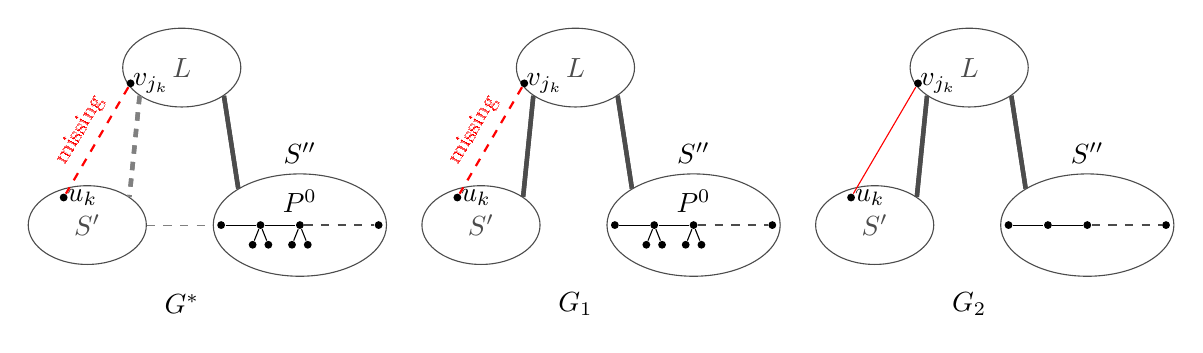
\begin{tikzpicture}[
    set/.style={ellipse, draw, minimum width=1.5cm, minimum height=1cm, opacity=0.7},
    node distance=1cm,
    point/.style={circle, fill=black, inner sep=1pt},
    label/.style={font=\small}
]

% Upper ellipse (L) - smaller and de-emphasized , fill=blue!10
\node[set] (L) at (0,2) {$L$};

\node[point, label=left:$v_{j_k}$] (vjk) at (-0.65,1.8) {};
\node[right=-0.15cm of vjk, align=center] {$v_{j_k}$};
% Lower left ellipse (S') - smaller and de-emphasized
\node[set] (S1) at (-1.2,0) {$S'$};
\node[point, label=left:$u_k$] (uk) at (-1.5,0.35) {};
\node[right=-0.13cm of uk, align=center] {$u_k$};
% Lower right ellipse (S'') - smaller and de-emphasized

 \node[set, minimum width=2.2cm, minimum height=1.3cm] (S2) at (1.5,0) {};
\node[above=0cm of S2, align=center] {$S''$};
%\node[set] (S2) at (1.5,0) {$S''$};

\node[point] (A1) at (0.5,0) {};
\node[point] (A2) at (1.0,0) {};
\node[point] (A3) at (1.5,0) {};
\node[point] (A4) at (2.5,0) {};
\draw[dashed, black!70,thick] (A3.east) -- (A4.west);
% 绘制四面体
\draw (A1) -- (A2)-- (A3);
\node[point] (A5) at (0.9,-0.25) {};
\node[point] (A6) at (1.1,-0.25) {};
\node[point] (A7) at (1.4,-0.25) {};
\node[point] (A8) at (1.6,-0.25) {};
\draw (A5) -- (A2)-- (A6);
\draw (A7) -- (A3)-- (A8);
\node at (1.5,0.3) {$P^0$};

% De-emphasized connections between L and S''
\foreach \i in {1,...,2} {
    \draw[black!70, ultra thick] (L.south east) -- (S2.north west);
    %\draw[black!50] (L.south) -- (S2.north);
}

% De-emphasized missing edges between L and S'
\foreach \i in {1,...,2} {
    \draw[dashed, black!50, ultra thick] (L.south west) -- (S1.north east);
    %\draw[dashed, black!50] (L.south) -- (S1.north);
}

% Highlighted missing edge between marked points
\draw[dashed, red, thick] (vjk) to node[label, sloped, above] {\footnotesize missing} (uk);

% Optional de-emphasized edges between S' and S''
\draw[dashed, black!50] (S1.east) -- (S2.west);
\node at (0,-1) {$G^*$};
%%%%%%%%%%%%%%%%%%

\node[set] (L) at (5,2) {$L$};
\node[point, label=left:$v_{j_k}$] (vjk) at (4.35,1.8) {};
\node[right=-0.15cm of vjk, align=center] {$v_{j_k}$};
% Lower left ellipse (S') - smaller and de-emphasized
\node[set] (S1) at (3.8,0) {$S'$};
\node[point, label=left:$u_k$] (uk) at (3.5,0.35) {};
\node[right=-0.13cm of uk, align=center] {$u_k$};
% Lower right ellipse (S'') - smaller and de-emphasized
\node[set, minimum width=2.2cm, minimum height=1.3cm] (S2) at  (6.5,0) {};
\node[above=0cm of S2, align=center] {$S''$};
%\node[set] (S2) at (6.5,0) {$S''$};
\node[point] (A1) at (5.5,0) {};
\node[point] (A2) at (6.0,0) {};
\node[point] (A3) at (6.5,0) {};
\node[point] (A4) at (7.5,0) {};
\draw[dashed, black!70,thick] (A3.east) -- (A4.west);
% 绘制四面体
\draw (A1) -- (A2)-- (A3);
\node[point] (A5) at (5.9,-0.25) {};
\node[point] (A6) at (6.1,-0.25) {};
\node[point] (A7) at (6.4,-0.25) {};
\node[point] (A8) at (6.6,-0.25) {};
\draw (A5) -- (A2)-- (A6);
\draw (A7) -- (A3)-- (A8);
\node at (6.5,0.3) {$P^0$};

% De-emphasized connections between L and S''
\foreach \i in {1,...,2} {
    \draw[black!70, ultra thick] (L.south east) -- (S2.north west);
    %\draw[black!50] (L.south) -- (S2.north);
}

% De-emphasized missing edges between L and S'
\foreach \i in {1,...,2} {
    \draw[black!70, ultra thick] (L.south west) -- (S1.north east);
    %\draw[dashed, black!50] (L.south) -- (S1.north);
}

% Highlighted missing edge between marked points
\draw[dashed, red, thick] (vjk) to node[label, sloped, above] {\footnotesize missing} (uk);

% Optional de-emphasized edges between S' and S''
%\draw[dashed, black!50] (S1.east) -- (S2.west);
\node at (5,-1) {$G_1$};
%%%%%%%%%%%%%%%%%%%%%%%%%%

\node[set] (L) at (10,2) {$L$};
\node[point, label=left:$v_{j_k}$] (vjk) at (9.35,1.8) {};
\node[right=-0.15cm of vjk, align=center] {$v_{j_k}$};
% Lower left ellipse (S') - smaller and de-emphasized
\node[set] (S1) at (8.8,0) {$S'$};
\node[point, label=left:$u_k$] (uk) at (8.5,0.35) {};
\node[right=-0.13cm of uk, align=center] {$u_k$};
% Lower right ellipse (S'') - smaller and de-emphasized

\node[set, minimum width=2.2cm, minimum height=1.3cm] (S2) at (11.5,0) {};
\node[above=0cm of S2, align=center] {$S''$};

\node[point] (A1) at (10.5,0) {};
\node[point] (A2) at (11.0,0) {};
\node[point] (A3) at (11.5,0) {};
\node[point] (A4) at (12.5,0) {};
\draw[dashed, black!70,thick] (A3.east) -- (A4.west);
% 绘制四面体
\draw (A1) -- (A2)-- (A3);
% De-emphasized connections between L and S''
\foreach \i in {1,...,2} {
    \draw[black!70, ultra thick] (L.south east) -- (S2.north west);
    %\draw[black!50] (L.south) -- (S2.north);
}

% De-emphasized missing edges between L and S'
\foreach \i in {1,...,2} {
    \draw[black!70, ultra thick] (L.south west) -- (S1.north east);
    %\draw[dashed, black!50] (L.south) -- (S1.north);
}

% Highlighted missing edge between marked points
%\draw[black, thick] (vjk) to node[label, sloped, above]  (uk);
\draw[red](vjk) -- (uk);
\node at (10,-1) {$G_2$};
% Optional de-emphasized edges between S' and S''
%\draw[dashed, black!50] (S1.east) -- (S2.west);

\end{tikzpicture}
    \caption{Graph transformations.}
    \label{fig:1}
\end{figure}
\begin{claim}\label{lem3.4}
If $e(L,S')\neq |L||S'|-1$, then $\rho(G_1)>\rho^*$.
\end{claim}
  \begin{proof}[\bf Proof of Claim \ref{lem3.4}]
Assume that $e(L,S')\neq |L||S'|-1$, that is,  $G^*[L,S']\neq G_1[L,S']$. Hence, either $|S'|\geq 2$ or $|S'|=1$ and $d_L(u_1)\leq\gamma_\mathbb{H}-2$.
Let $k'$ be an integer in $[|S'|]\setminus \{k\}$ if $|S'|\geq 2$, and let $k'=1$ otherwise. Recall that $x_v\geq (1-\frac{1}{(10C_\mathbb{H})^2})x_{u^*}\geq\frac{1}{2}x_{u^*}$ for each $v\in L$.  It is routine to check that \allowdisplaybreaks
    \begin{align*}\notag
        \rho(G_1)-\rho^* \geq& {\bf x}^T\left(A(G_1)-A(G^*)\right){\bf x}\\
        =&\sum_{i=1}^{|S'|}2x_{u_i}\left(\sum_{v\in L_i}x_v-\sum_{v\in N_{S'_{i}}(u_i)}x_v-\sum_{v\in N_{S''}(u_i)}x_v\right)-2x_{u_k}x_{v_{j_k}}\\
        \geq&\sum_{i\in [|S'|]\setminus \{k,k'\}}2x_{u_i}\left(\sum_{v\in L_i}x_v-\sum_{v\in N_{S'_{i}}(u_i)}x_v-\sum_{v\in N_{S''}(u_i)}x_v\right)\\
        &+2x_{u_{k'}}\left(\frac{1}{2}x_{u^*}-\sum_{v\in  N_{S'_{k'}}(u_{k'})}x_v-\sum_{v\in  N_{S''}(u_{k'})}x_v-\sum_{v\in N_{S'_{k}}(u_k)}x_v-\sum_{v\in N_{S''}(u_k)}x_v\right).
    \end{align*}

Together with Lemmas~\ref{lem3.1}-\ref{lem3.2}, for each $i\in [|S'|]\setminus \{k,k'\}$ one has 
\begin{align*}
    \sum_{v\in L_i}x_v-\sum_{v\in N_{S'_{i}}(u_i)}x_v-\sum_{v\in N_{S''}(u_i)}x_v
    \geq\frac{1}{2}x_{u^*}-2C_\mathbb{H}\frac{x_{u^*}}{20C_\mathbb{H}}-\max_{H\in \mathbb{H}}\{|H|\}\frac{x_{u^*}}{20C_\mathbb{H}}
    >0,
\end{align*}
and similarly 
\begin{align*}
   &\frac{1}{2}x_{u^*}-\sum_{v\in  N_{S'_{k'}}(u_{k'})}x_v-\sum_{v\in  N_{S''}(u_{k'})}x_v-\sum_{v\in N_{S'_{k}}(u_k)}x_v-\sum_{v\in N_{S''}(u_k)}x_v>0.%\\    \geq&\frac{1}{2}x_{u^*}-4C_H\frac{x_{u^*}}{20C_H}-2|H|\frac{x_{u^*}}{20C_H}    >0
\end{align*}
If $\max\{x_{u_i}:i\in [|S'|]\}>0$, then $\rho(G_1)>\rho^*$, as desired. If $x_{u_1}=\cdots=x_{u_{|S'|}}=0$, then each vertex in $S'$ is not adjacent to any vertex in $L\cup S''$, that is, $G^*[L\cup S'']$ is a connected component of $G^*$. Furthermore, $\rho(G^*[L\cup S''])=\rho^*$.  However, $G^*[L\cup S'']$ is a proper subgraph of some connected component of $G_1$. Hence, $\rho(G_1)>\rho^*$, as desired.
 \end{proof}

A \textit{linear path} in a graph $G$ is a path where every internal vertex along the path has degree exactly $2$ in $G$, while the endpoints may  coincide (forming a cycle). 
Denote $\zeta:=\max_{H\in \mathbb{H}}\{2|H|^2\}$. Based on Lemma~\ref{lem3.3}, we know that $S''$ contains a path $P$ of  order at least $\zeta$. % for some  $H\in\mathbb{H}$. 
Let $P^0=w_1w_2\ldots w_{\zeta}$ be a subpath of $P$. 
Notice that $P^0$ may not be a linear path.
Let $G_2$ be the graph obtained from $G_1+\{u_kv_{j_k}\}$ by deleting all edges within $S''$ that are incident to some vertices in $P^0$ but do not belong to $E(P^0)$  (see Figure \ref{fig:1}). 
Next, we compare the spectral radii of $G_2$ and $G^*$. 

\begin{claim}\label{lem3.5}
 $\rho(G_2)>\rho^*$. 
\end{claim}
\begin{proof}[\bf Proof of Claim \ref{lem3.5}]
    Let ${\bf y}=(y_1,y_2,\ldots,y_n)^{T}$ be a non-negative unit eigenvector of 
$A(G_1)$ with respect to $\rho(G_1)$, and let ${\bf z}=(z_1,z_2,\ldots, z_n)^T$ be a non-negative unit eigenvector of $A(G_2)$ with respect to $\rho(G_2)$. Let %$y_{u^*}:=\max_{w\in V}y_w$, 
    $y_{S''}^*:=\max_{w\in S''}y_w$,  $\sigma_L:=\sum_{u\in L}y_u$, and let $z_{S''}^*=\max_{u\in S''}z_u$. 
We proceed by  considering the following two cases.

{\bf Case 1.} $e_{G^*}(L,S')\neq |L||S'|-1$.
    
    In view of Claim~\ref{lem3.4}, we have $\rho(G_1)>\rho^*$, so it suffices to prove $\rho(G_2)>\rho(G_1)$. Notice that $\rho(G_1)y_{S''}^*\leq \alpha_{\mathbb{H}}y_{S''}^*+\sigma_L$, this implies 
    \begin{align}\label{ys}
        y_{S''}^*\leq \frac{\sigma_L}{\rho(G_1)-\alpha_{\mathbb{H}}}.
    \end{align}
        %\rho(G_1)y_w=\underset{u\in N_{G_1}(w)}{\sum}y_u=\underset{u\in N_{L\cup S''}(w)}{\sum}y_u+\underset{u\in N_{S'}(w)}{\sum}y_u\leq C_Hy_{u^*}+\frac{\gamma_Hn}{100C_H\rho(G_1)}y_{u^*}%\leq C_Hy_{u^*}+\frac{3\gamma_Hn}{100C_H\rho(G_1)}y_{u^*}.
  

By the construction of
$G_1$, we have $|E(G_1)|\leq |E(G^*)|+|L||S'|\leq C_\mathbb{H} n+\frac{\gamma_\mathbb{H}^2n}{(10C_\mathbb{H})^2}$. Together with the well-known fact that 
$\rho(G_1)\leq \sqrt{2|E(G_1)|}$, we have 
$$
\sqrt{2\left(C_\mathbb{H} n+\frac{\gamma_\mathbb{H}^2n}{(10C_\mathbb{H})^2}\right)}\rho(G_1)y_{v_{j_k}}\geq \rho(G_1)^2y_{v_{j_k}}\geq \sum_{u\in S\setminus \{u_k\}}\rho(G_1)y_u\geq (|S|-1)\sigma_L=(n-\gamma_\mathbb{H}-1)\sigma_L.
$$
It follows that 
\begin{align}\notag
    y_{v_{j_k}}&\geq \frac{(n-\gamma_\mathbb{H}-1)\sigma_L}{\rho(G_1)\sqrt{2\left(C_\mathbb{H} n+\frac{\gamma_\mathbb{H}^2n}{(10C_\mathbb{H})^2}\right)}}\\\notag
    &\geq \frac{\sigma_L}{\rho(G_1)-\alpha_{\mathbb{H}}}\cdot\frac{n-\gamma_\mathbb{H}-1}{2\sqrt{C_\mathbb{H} n+\frac{\gamma_\mathbb{H}^2n}{(10C_\mathbb{H})^2}}}\\\label{eq:4.1}
    &>\frac{\sigma_L\cdot 4\zeta\alpha_{\mathbb{H}}}{\rho(G_1)-\alpha_{\mathbb{H}}}\geq 4\zeta\alpha_{\mathbb{H}}y_{S''}^*.
\end{align}

    We first assume that $\gamma_\mathbb{H}\geq2$. Clearly, 
    \begin{align}\notag\label{eq:4}
        \rho(G_2)-\rho(G_1)&\geq{\bf y}^T\left(A(G_2)-A(G_1)\right){\bf y}\\&\geq 2y_{v_{j_k}}y_{u_k}-2\sum_{i=1}^{\zeta}\sum_{w\in N_{S''}(w_i)}y_{w_i}y_w.
    \end{align}
We claim that $\sigma_L\geq 2y_{v_{j_k}}$. In fact, if $y_{v_{j_k}}\leq y_{v_{\ell}}$ for some $\ell\neq j_k$, then $\sigma_L\geq 2y_{v_{j_k}}$. If $y_{v_{j_k}}> y_{v_{\ell}}$ for every  $\ell\neq j_k$, then $N_L(v_{j_k})\neq \emptyset$ and  
$$
\rho(G_1)\left(\sum_{v_\ell\in N_L(v_{j_k})}y_{v_\ell}-y_{v_{j_k}}\right)\geq |N_L(v_{j_k})|y_{v_{j_k}}-\sum_{v_\ell\in N_L(v_{j_k})}y_{v_\ell}>0.
$$
Therefore, $\sigma_L\geq 2y_{v_{j_k}}$, as desired. 
Notice that $\rho(G_1)y_{u_k}=\sigma_L-y_{v_{j_k}}$, % and  $\rho(G_1)y_{S''}^*\leq\sigma_L+\alpha_Hy_{S''}^*$ for each $H\in\mathbb{H}$, 
which combined with \eqref{ys}, implies that  
\begin{align*}
y_{S''}^*\leq\frac{\sigma_L}{\rho(G_1)-\alpha_\mathbb{H}}\leq\frac{2(\sigma_L-y_{v_{j_k}})}{0.5\rho(G_1)}=4y_{u_k}.
\end{align*}
   Therefore, %for each $H\in\mathbb{H}$,
    \begin{align*}
        \sum_{i=1}^{\zeta}\sum_{w\in N_{S''}(w_i)}y_{w_i}y_w\leq\zeta\alpha_\mathbb{H}\cdot y_{S''}^*\cdot4y_{u_k}=4\zeta\alpha_\mathbb{H}\cdot y_{S''}^*y_{u_k}.
    \end{align*}
Combining this with \eqref{eq:4.1} and \eqref{eq:4}, we get that $\rho(G_2)-\rho(G_1)>0$, as desired. 
    
    Next, we assume that $\gamma_\mathbb{H}=1$ and $v_1 (=v_{j_k})$ is the unique vertex in $L$.
%Recall that ${\bf z}=(z_1,z_2,\ldots,  z_n)^T$ is a non-negative unit eigenvector of $A(G_2)$ with respect to $\rho(G_2)$.
    Notice that $\rho(G_2)z_{S''}^*\leq z_{v_1}+\alpha_\mathbb{H}z_{S''}^*$ %for each $H\in\mathbb{H}$
    and $\rho(G_2)z_{u_k}=z_{v_1}$. 
    This yields $(\rho(G_2)-\alpha_\mathbb{H})z_{S''}^*\leq \rho(G_2)z_{u_k}$, % for each $H\in\mathbb{H}$ , 
    which implies $z_{S''}^*\leq 2z_{u_k}$. Combining this with \eqref{eq:4.1}, one has 
    %Using the same method in~\eqref{eq2}, we have $z_{S''}^*<\frac{z_{u^*}}{20C_H}$.
    %Thus,
    \begin{align*}
        {\bf y}^T{\bf z}(\rho(G_2)-\rho(G_1))&={\bf y}^T\left(A(G_2)-A(G_1)\right){\bf z}\\
        &=y_{u_k}z_{v_1}+y_{v_1}z_{u_k}-\sum_{i=1}^{\zeta}\sum_{w\in N_{S''}(w_i)}(y_{w_i}z_w+y_wz_{w_i})\\&\geq y_{v_1}z_{u_k}-2\zeta\cdot\alpha_\mathbb{H}\cdot y_{S''}^*z_{S''}^*\\&>0.%\geq y_{v_1}z_{u_k}\left(1-\frac{1}{20C_H}\cdot8|H|^2\alpha_H\right)\\&>0
    \end{align*}
That is, $\rho(G_2)>\rho(G_1)$, as desired. 

{\bf Case 2.} $e_{G^*}(L,S')=|L||S'|-1$.

In this case, $S'=\{u_1\}$ and $d_L(u_1)=\gamma_\mathbb{H}-1$. 
    %Recall that ${\bf x}=(x_1,x_2,\ldots, x_n)^T$ is a non-negative unit eigenvector of $G^*$ corresponding to $\rho^*$ and ${\bf z}=(z_1,z_2\ldots z_n)^T$ is a non-negative unit eigenvector of $A(G_2)$ with respect to $\rho(G_2)$. Define $z_{S''}^*:=\max_{w\in S''}z_w$. 
    Notice that $\rho(G_2)z_{u_1}=\sum_{w\in L}z_w$ and $\rho(G_2)z_{S''}^*\leq\sum_{w\in L}z_w+\alpha_\mathbb{H}z_{S''}^*$, % for each $H\in\mathbb{H}$, 
    which implies $z_{S''}^*\leq 2z_{u_1}$. Recall that $x_{v_{j_1}} \geq \left(1-\frac{1}{2(10C_\mathbb{H})^{2}}\right)x_{u^{*}}$.  Together with Lemmas~\ref{lem3.1}-\ref{lem3.2} and the choice of $C_\mathbb{H}$, one has
    \begin{align*}
        {\bf x}^T{\bf z}(\rho(G_2)-\rho^*)&={\bf x}^T(A(G_2)-A(G^*)){\bf z} \\&\geq x_{u_1}z_{v_{j_1}}+x_{v_{j_1}}z_{u_1}-\sum_{i=1}^{\zeta}\sum_{w\in N_{S''}(w_i)}(x_{w_i}z_w+x_wz_{w_i})-\sum_{w\in N_{S''}(u_1)}(x_{u_1}z_w+x_wz_{u_1})\\ &\geq x_{v_{j_1}}z_{u_1}-2\zeta\cdot \alpha_\mathbb{H}\cdot x_{S''}^*z_{S''}^*-\zeta \cdot x_{S''}^*z_{S''}^*\\ &\geq \frac{1}{2}x_u^*z_{u_1}-3\zeta\cdot  \alpha_\mathbb{H}\cdot\frac{x_u^*}{20C_\mathbb{H}}\cdot2z_{u_1}\\ &>0.
    \end{align*}
That is, $\rho(G_2)>\rho^*$, as desired. 
\end{proof}

Based on Claim~\ref{lem3.5} and the fact that $G^*\in {\rm SPEX}(n,\mathbb{H}_{\rm sub})$, we know that $G_2$ contains an $H$-subdivision for some $H\in\mathbb{H}$.
    Choose a minimal $H$-subdivision in $G_2$, say $H_S$, such that it contains as many vertices as possible in $S''$.
    Assume that $(P^1,\ldots,P^{m})$ is the corresponding $H$-partition of $H_S$, where $m=e(H)$. 
    
    Applying a similar discussion as Lemma \ref{lem3.3} yields that $S''\subseteq V(H_S)$. Recall that $P^0$ is a linear path inside $G_2$. Thus, $|V(P^i)\cap V(P^0)|\leq 2$ for every $i\in [m]$, which implies that at most $2m<2|H|^2\leq \zeta$ vertices in $P^0$ appear in $H_S$, a contradiction. 
    %We choose a minimal one $H_s$.     As $H_s$ is a minimal $H$-subdivision, it contains all vertices in $S''$, including $P_0$.     But since $P_0$ is a linear path, we know that two consecutive vertices on $P_0$ do not belong to the same $V_{E_i}$.     So $H_s$ only uses $|H|+\dbinom{|H|}{2}<2|H|^2$ vertices in $P_0$ at most, a contradiction.     This completes the proof that $S'=\emptyset$.
\end{proof}

In the following, we complete the proof of Theorem~\ref{thm1.3}.
\begin{proof}[\bf Proof of Theorem \ref{thm1.3}]
Based on Lemma~\ref{lem2.4} and  Lemma~\ref{lem3.6}, we know that $V(G^*)=L\cup S$ with $|L|=\gamma_\mathbb{H}$ and $G^*[L,S]=K_{\gamma_\mathbb{H},n-\gamma_\mathbb{H}}$. Hence, in order to prove that $G^*$ contains $B_{\gamma_\mathbb{H},n-\gamma_\mathbb{H}}$ as a spanning subgraph, it suffices to show $G^*[L]\cong K_{\gamma_\mathbb{H}}$.

    Suppose to the contrary that $G^*[L]$ is not a clique. Without loss of generality, assume that $v_1v_2\notin E(G^*)$. 
    Since $|S|=n-|L|>\max_{H\in \mathbb{H}}\{2|H|^2\}=:\zeta$, one may choose a subset $T\subseteq S$ with $|T|=\zeta$.
    Let $T':=S\setminus T$.
    By Lemma~\ref{lem3.1}, $d_{S}(w)\leq\alpha_\mathbb{H}$ for each $w\in S$.
    It follows that %for each $H\in\mathbb{H}$
    \begin{align*}
        e(S)-e(T')\leq \sum_{v\in T}d_{S''}(v)\leq \alpha_\mathbb{H}\zeta.
    \end{align*}
    Moreover, let $x_{S}^*:=\max_{w\in S}x_w$.
    Then $\rho^*x_{S}^*\leq\sum_{u\in L}x_u+\alpha_\mathbb{H}x_{S}^*$. Recall that $\rho^*\geq \sqrt{\gamma_\mathbb{H}(n-\gamma_\mathbb{H})}$.
    Hence,
    \begin{align*}
        x_{S}^*\leq\frac{\sum_{u\in L}x_u}{\rho^*-\alpha_\mathbb{H}}\leq\frac{\gamma_\mathbb{H}x_{u^*}}{\rho^*-\alpha_\mathbb{H}}\leq\sqrt{\frac{2\gamma_\mathbb{H}}{n}}x_{u^*}.
    \end{align*}

    Let $G$ be a graph obtained from $G^*+v_1v_2$ by removing all edges in $E(G^*[S])\setminus E(G^*[T'])$.
    By Lemma~\ref{lem2.4}, one has $\min\{x_{v_1},x_{v_2}\}\geq(1-\frac{1}{2(10C_\mathbb{H})^2})x_{u^*}$. Thus, as $n$ is sufficiently large, one has 
    \begin{align*}
        \rho(G)-\rho^*&\geq {\bf x}^T\left(A(G)-A(G^*)\right){\bf x}\\
        &\geq 2\left(x_{v_1}x_{v_2}-\sum_{w_1w_2\in E(G^*[S])\setminus E(G^*[T'])}x_{w_1}x_{w_2}\right)\\&\geq 2\left(\left(1-\frac{1}{2(10C_\mathbb{H})^2}\right)^2-\frac{\alpha_\mathbb{H}\zeta\cdot 2\gamma_\mathbb{H}}{n}\right)x_{u^*}^2\\&>0, 
    \end{align*}
    which implies that $\rho(G)>\rho^*$. Therefore, $G$ has an $H$-subdivision for some $H\in\mathbb{H}$, containing the edge $v_1v_2$. Choose a minimum  $H$-subdivision in $G$, say $H_S$. Assume that $(P^1,\ldots,P^{m})$ is the corresponding $H$-partition of $H_S$, where $m=e(H)$.

   Notice that $G[T]$ is an empty graph. By the minimality of $H_S$, we know that $|V(P^i)\cap T|\leq 2$ for each $i\in [m]$. Hence at least one vertex, say $w\in S$, does not appear in $H_S$. Consequently, $H_{S}$ is also an $H$-subdivision of $G-w$.
    Now, replace the edge $v_1v_2$ in $H_S$ with a three-vertex path $v_1wv_2$, which also forms an $H$-subdivision. It follows that $G^*$ contains an $H$-subdivision, a contradiction.
    
    This completes the proof of Theorem~\ref{thm1.3}.
\end{proof}


\section{Proof of Lemma \ref{lem2.4}}\label{sec4}

In this section, we give the proof of Lemma \ref{lem2.4}. Let $n$ be a sufficiently large integer and $\mathbb{H}$ be a family of graphs with $\gamma_{\mathbb{H}}\geq 1$.  Assume that $G$ is an $n$-vertex $\mathbb{H}$-subdivision-free graph with $\rho(G) \geq \sqrt{\gamma_\mathbb{H}(n-\gamma_\mathbb{H})}$.  Let ${\bf x}$ be a non-negative unit eigenvector of $A(G)$ corresponding to $\rho(G)$ and  $u^{*} \in V(G)$ be a vertex satisfying $x_{u^{*}}=\max_{u \in V(G)}x_{u}$.
To prove Lemma~\ref{lem2.4}, our goal is to find a set $L$ of exactly $\gamma_\mathbb{H}$ vertices in $G$ such that $x_{u} \geq (1-\frac{1}{2(10C_\mathbb{H})^{2}})x_{u^{*}}$ and $d_{G}(u) \geq (1-\frac{1}{(10C_\mathbb{H})^{2}})n$ for every $u \in L$.
For a positive integer $\lambda$,  define %We first define a subset of $V(G)$ as follows:
$$
L^\lambda=\{u\in V(G):x_{u}\geq (10C_\mathbb{H})^{-\lambda}x_{u^*}\}. 
$$
We adhere to the high-level methodological framework outlined in \cite{byrne2024general}:
\begin{enumerate}
%    \item Show that $|L^{\lambda}|$ is not too large for every integer $\lambda$;
    \item Show that $|L^4|$ is in fact bounded;
    \item Relate the eigenweight of vertices in $L^4$ to their degrees;
    \item Show that eigenweights of vertices in $L^1$  are close to $1$;
    \item Show that $|L^1|=k$.
\end{enumerate}
%where $\lambda$ is a positive integer.

For a vertex $u\in V(G)$ and a positive integer $i$, let $N_i(u)$ be the set of vertices at distance $i$ from $u$ in $G$.
We will frequently use $N_1(u)$ and $N_2(u)$ below.
Furthermore, we use $L_i^\lambda(u)$ and $\overline{L}_i^\lambda(u)$ to denote $N_i(u)\cap L^\lambda$ and $N_i(u)\setminus L^\lambda$, respectively.
When the reference vertex $u$  is clear from context, we shall omit it and simply write $L_i^\lambda$ and $\overline{L}_i^\lambda$ respectively. 
%When there is no ambiguity, we use $L_i^\lambda$ and $\overline{L}_i^\lambda$ to represent $L_i^\lambda(u)$ and $\overline{L}_i^\lambda(u)$, respectively.
We also denote $L_{i,j}^\lambda=L_i^\lambda \cup L_j^\lambda$ and $\overline{L}_{i,j}^\lambda=\overline{L}_i^\lambda \cup \overline{L}_j^\lambda$ for simplicity.

\begin{proof}[\bf Proof of Lemma \ref{lem2.4}]
%We now establish some claims on $L^{\lambda}$.
With the above notation established, we are to find a set $L$ of exactly $\gamma_\mathbb{H}$ vertices in $G$ such that $x_{u} \geq (1-\frac{1}{2(10C_\mathbb{H})^{2}})x_{u^{*}}$ and $d_{G}(u) \geq (1-\frac{1}{(10C_\mathbb{H})^{2}})n$ for every $u \in L$. We first show an inequality for $\gamma_{\mathbb{H}}^2$. 


\begin{claim}\label{lem4.2}
    For every vertex \( u \in V(G) \) and every positive integer \( \lambda \), we have 
    \begin{align}\label{eq:5}
        \gamma_\mathbb{H}(n-\gamma_\mathbb{H})x_u \leq |N_1(u)|x_u + \left( \frac{2C_\mathbb{H}n}{(10C_\mathbb{H})^{10-\lambda}} + \frac{2C_\mathbb{H}n}{(10C_\mathbb{H})^\lambda} \right)x_{u^*} + \sum_{\substack{v \in \overline{L}_1^\lambda,\,w \in N_{L_{1,2}^\lambda}(v)}} x_w.
    \end{align}
\end{claim}

\begin{proof}[\bf Proof of Claim \ref{lem4.2}]
    Recall that \( \rho(G) \geq \sqrt{\gamma_\mathbb{H}(n-\gamma_\mathbb{H})} \). Hence 
    \begin{align}\notag
        \gamma_\mathbb{H}(n-\gamma_\mathbb{H})x_u \leq \rho(G)^2x_u &= |N_1(u)|x_u + \sum_{\substack{v \in N_1(u),\,w \in N_1(v)\setminus\{u\}}} x_w\\\label{eq:6}
        &= |N_1(u)|x_u + \sum_{v\in L_1^\lambda \cup \overline{L}_1^\lambda}\,\sum_{\substack{w \in N_{L_{1,2}^\lambda}(v) \cup N_{\overline{L}_{1,2}^\lambda}(v)}} x_w.
    \end{align}   
%    For each \( v \in N_1(u) \), decompose \( N_1(v)\setminus\{u\} \) into
  %  \[
  %  N_1(v)\setminus\{u\} = N_{L_{1,2}^\lambda}(v) \cup N_{\overline{L}_{1,2}^\lambda}(v),
   % \]
   % where \( N_{L_{1,2}^\lambda}(v) \subseteq \bigcup_{i=1}^2 L_i^\lambda \cup \overline{L}_i^\lambda \). 
   % Partition \( N_1(u) = L_1^\lambda \cup \overline{L}_1^\lambda \). For \( v \in L_1^\lambda \), we have
   By the definition of \( L^\lambda \), vertices in \( \overline{L}_{1,2}^\lambda \) satisfy \( x_w < (10C_\mathbb{H})^{-\lambda}x_{u^*} \). Hence 
    \begin{align}\notag
        %\sum_{\substack{v \in L_1^\lambda, \\ w \in N_1(v)\setminus\{u\}}} x_w &\leq 
        \sum_{v \in L_1^\lambda}\left(\sum_{w \in N_{L_{1,2}^\lambda}(v)} x_w + \sum_{w \in N_{\overline{L}_{1,2}^\lambda}(v)} x_w\right) 
        \leq &\sum_{v \in L_1^\lambda}\left(\sum_{w \in N_{L_{1,2}^\lambda}(v)} x_{u^*} + \sum_{w \in N_{\overline{L}_{1,2}^\lambda}(v)} (10C_\mathbb{H})^{-\lambda}x_{u^*}\right) \\\label{eq:7}
        \leq &\left(2e(L_1^\lambda) + e(L_1^\lambda, L_2^\lambda)\right)x_{u^*} + e\left(L_1^\lambda, \overline{L}_{1,2}^\lambda\right)(10C_\mathbb{H})^{-\lambda}x_{u^*},
    \end{align}
 and similarly, 
    \begin{align}\label{eq:8}
        \sum_{v \in \overline{L}_1^\lambda}\sum_{w \in N_{\overline{L}_{1,2}^\lambda}(v)} x_w\leq  \left(2e(\overline{L}_1^\lambda) + e(\overline{L}_1^\lambda, \overline{L_2^\lambda})\right)(10C_\mathbb{H})^{-\lambda}x_{u^*}.
    \end{align}
Together with Theorem~\ref{lem2.1} and the fact that $G$ is $\mathbb{H}$-subdivision-free, one has % we can bound edge terms:
    \[
    2e(L_1^\lambda) + e(L_1^\lambda, L_2^\lambda) \leq 2C_\mathbb{H}|L^\lambda|, \quad \text{and} \quad e\left(L_1^\lambda, \overline{L}_{1,2}^\lambda\right) + 2e(L_1^\lambda) + e\left(\overline{L}_1^\lambda, \overline{L}_2^\lambda\right) < 2C_\mathbb{H}n.
    \]
    
Now, we consider the size of $|L^{\lambda}|$. Note that  $\rho(G) \geq \sqrt{\gamma_\mathbb{H}(n-\gamma_\mathbb{H})}>2C_\mathbb{H}(10C_\mathbb{H})^{10}$ as $n$ is sufficiently large and $x_u \geq (10C_\mathbb{H})^{-\lambda}x_{u^*}$ for every $u\in L^{\lambda}$. Then  
    \[
    |L^{\lambda}|2C_\mathbb{H}(10C_\mathbb{H})^{10-\lambda}x_{u^*} \leq \sum_{u\in L^{\lambda}}\rho(G)x_u = \sum_{u\in L^{\lambda}}\sum_{v \in N_1(u)} x_v \leq \sum_{u\in L^{\lambda}}|N_1(u)|x_{u^*}\leq 2e(G)x_{u^*} < 2C_\mathbb{H}nx_{u^*}.
    \]
    %This implies \(2C_\mathbb{H}(10C_\mathbb{H})^{10-\lambda} < |N_1(u)|\) for all \(u \in L^\lambda\). Summing over \(L^\lambda\) and applying Theorem~\ref{lem2.1}, we get
    %\[
    %2C_\mathbb{H}(10C_\mathbb{H})^{10-\lambda}|L^\lambda| < \sum_{u \in L^\lambda} |N_1(u)| \leq 2e(G) < 2C_\mathbb{H}n.
    %\]
    It follows that for every 
integer $\lambda$ we have
\begin{align}\label{eq:n01}
    |L^\lambda| < (10C_\mathbb{H})^{\lambda-10}n.
\end{align}
    %which directly simplifies to the claimed bound. 
    By substituting \eqref{eq:7}-\eqref{eq:n01} into \eqref{eq:6}, we obtain our desired inequality immediately. % yields \eqref{eq:5}.
%    By Claim~\ref{lem4.1}, \( |L^\lambda| < (10C_\mathbb{H})^{\lambda-10}n \). Substituting these into \eqref{eq:6}-\eqref{eq:8} yields \eqref{eq:5}.
\end{proof}
    
    Next, we show that $|L^4|$ is bounded. %, which depends only on $C_\mathbb{H}$.
   
\begin{claim}\label{lem4.3}
    $|L^4| < (10C_\mathbb{H})^6$.
    \end{claim}

\begin{proof}[\bf Proof of Claim \ref{lem4.3}]
    Suppose, for contradiction, that there exists \( u_0 \in L^4 \) such that \( |N_1(u_0)| < (10C_\mathbb{H})^{-5}n \). Substituting \( \lambda = 5 \) in \eqref{eq:5} gives that
    \begin{align}\notag
        \gamma_\mathbb{H}(n-\gamma_\mathbb{H})x_{u_0} &\leq |N_1(u_0)|x_{u_0} +  \frac{4C_\mathbb{H}n}{(10C_\mathbb{H})^{5}} x_{u^*} + e(\overline{L}_1^5, L_{1,2}^5) x_{u^*}\\\notag
        &\leq \left((10C_\mathbb{H})^{-5}n+\frac{4C_\mathbb{H}n}{(10C_\mathbb{H})^{5}}+C_\mathbb{H}(|N_1(u_0)| + |L^5|)\right)x_{u^*}\\\label{eq111}
        &\leq \frac{(1+6C_\mathbb{H})n}{(10C_\mathbb{H})^5}x_{u^*},
        %\left(|N_1(u_0)| + \underbrace{e(\overline{L_1^5}, L_{1,2}^5)}_{\leq C_\mathbb{H}(|N_1(u_0)| + |L^5|)}\right)x_{u^*} \leq \frac{(1+2C_\mathbb{H})n}{(10C_\mathbb{H})^5}x_{u^*},
    \end{align}
 the last inequality holds by \eqref{eq:n01}. %   where Theorem~\ref{lem2.1} bounds edge counts and \eqref{eq:n01} gives \( |L^5| \leq (10C_\mathbb{H})^{-5}n \).

    On the other hand, since \( \gamma_\mathbb{H} \geq 1 \) and \( x_{u_0} \geq (10C_\mathbb{H})^{-4}x_{u^*} \), we have
    \[
    \gamma_\mathbb{H}(n-\gamma_\mathbb{H})x_{u_0} \geq \frac{7}{10}nx_{u_0} \geq 7C_\mathbb{H}(10C_\mathbb{H})^{-5}nx_{u^*},
    \]
    which contradicts~\eqref{eq111}. Thus \( |N_1(u)| \geq (10C_\mathbb{H})^{-5}n \) for all \( u \in L^4 \).
    Summing this over \( L^4 \) and applying Theorem~\ref{lem2.1} yields 
    \[
    |L^4|(10C_\mathbb{H})^{-5}n \leq \sum_{u \in L^4} |N_1(u)| < 2C_\mathbb{H}n.
    \]
    Thus,  $|L^4| < (10C_\mathbb{H})^6$, as desired.
\end{proof}
  We now estimate the degrees of vertices in $L^4$
  with respect to their eigenweights.%  Relate the eigenweight of vertices in $L^4$ to their degrees
\begin{claim}\label{lem4.4}
    For each \( u \in L^4 \), we have 
    $|N_1(u)| \geq \left(\frac{x_u}{x_{u^*}} - \frac{1}{(10C_\mathbb{H})^3}\right)n$.
    \end{claim}

\begin{proof}[\bf Proof of Claim \ref{lem4.4}]
    Given a vertex $u\in L^4$, let $L_0=\{v\in \overline{L}_1^4: |N(v)\cap L_{1,2}^4|\geq \gamma_{\mathbb{H}}\}$ and $H^*$ be a minimal  graph with respect to $\mathbb{H}$. % \( L_0 \subseteq \overline{L}_1^4 \) contain vertices with \(\geq \gamma_\mathbb{H}\) neighbors in \( L_{1,2}^4 \). 
    We first claim that %for each $H\in\mathbb{H}$, 
    $|L_0|\leq \eta(\alpha_\mathbb{H}+\binom{|H^*|+1}{2})$, where $\eta:=\binom
    {|L_{1,2}^4|}{\gamma_\mathbb{H}}$.
    In fact, if $|L_{1,2}^4|\leq \gamma_\mathbb{H}-1$, then $L_0=\emptyset$ and we are done.
    Now we  consider the case $|L_{1,2}^4|\geq\gamma_H$.
    Suppose in contrast that $|L_0|>\eta(\alpha_\mathbb{\mathbb{H}}+\binom{|H^*|+1}{2})$.
    Since there are only $\eta$ options for vertices in $L_0$ to choose $\gamma_\mathbb{H}$ neighbors from $L_{1,2}^4$, we can find $\gamma_\mathbb{H}$ vertices in $L_{1,2}^4$ with at least $|L_0|/\eta>\alpha_\mathbb{H}+\binom{|H^*|+1}{2}$ common neighbors in $L_0$.
    Furthermore, $u\notin L_{1,2}^4$ and $L_0\subseteq \overline{L}_1^4\subseteq N_1(u)$.
    Hence $u$ and those $\gamma_\mathbb{H}$ vertices have $\alpha_\mathbb{H}+\binom{|H^*|+1}{2}$ common neighbors, which implies that $G$ contains a bipartite subgraph $G[S,T]$ isomorphic to $K_{\gamma_\mathbb{H}+1,\alpha_\mathbb{H}+\binom{|H^*|+1}{2}}$. Thus, by Lemma~\ref{lem2.2}, $G$ contains an $H^*$-subdivision, a contradiction. 
    Therefore, $|L_0|\leq \eta(\alpha_\mathbb{H}+\binom{|H^*|+1}{2})$.
    
    By Claim~\ref{lem4.3} and the definition of $L_0$, we have %\[
    %e(L_0, L_{1,2}^4) \leq |L_0||L^4|\leq (10C_\mathbb{H})^{-4}n \quad \text{and} \quad e(\overline{L}_1^4\setminus L_0, L_{1,2}^4) \leq |N_1(u)|(\gamma_\mathbb{H}-1)
    %\]
%It follows that 
    \begin{align}\label{eq:10}
        e(\overline{L}_1^4, L_{1,2}^4) =e(L_0, L_{1,2}^4)+e(\overline{L}_1^4\setminus L_0, L_{1,2}^4) \leq (10C_\mathbb{H})^{-4}n+|N_1(u)|(\gamma_\mathbb{H}-1).
    \end{align}
    Substituting \(\lambda = 4\) in 
    \eqref{eq:5} yields \allowdisplaybreaks
    \begin{align*}
    \gamma_\mathbb{H}(n-\gamma_\mathbb{H})x_u &\leq |N_1(u)|x_u + \left( \frac{2C_\mathbb{H}n}{(10C_\mathbb{H})^{6}} + \frac{2C_\mathbb{H}n}{(10C_\mathbb{H})^4} \right)x_{u^*} + \sum_{\substack{v \in \overline{L}_1^4,\,w \in N_{L_{1,2}^4}(v)}} x_w\\
    &\leq \left(|N_1(u)| +  \frac{3C_\mathbb{H}n}{(10C_\mathbb{H})^{4}}+e(\overline{L}_1^4, L_{1,2}^4)\right)x_{u^*}\\
    &\leq \left(|N_1(u)| +  \frac{4C_\mathbb{H}n}{(10C_\mathbb{H})^{4}}+|N_1(u)|(\gamma_\mathbb{H}-1)\right)x_{u^*}\\
    &\leq \gamma_{\mathbb{H}}\left(|N_1(u)| +  \frac{4C_\mathbb{H}n}{(10C_\mathbb{H})^{4}}\right)x_{u^*}.
    \end{align*}
    This implies 
    \[
    |N_1(u)| \geq (n-\gamma_{\mathbb{H}})\frac{x_u}{x_{u^*}}-\frac{4C_\mathbb{H}n}{(10C_\mathbb{H})^{4}}=\left(\frac{x_u}{x_{u^*}}-\frac{4C_\mathbb{H}}{(10C_\mathbb{H})^{4}}\right)n-\gamma_{\mathbb{H}}\frac{x_u}{x_{u^*}}\geq \left(\frac{x_u}{x_{u^*}}-\frac{1}{(10C_\mathbb{H})^{3}}\right)n, 
    \]
    the last inequality holds as $\gamma_{\mathbb{H}}\frac{x_u}{x_{u^*}}\leq \gamma_{\mathbb{H}}\leq \frac{6C_\mathbb{H}n}{(10C_\mathbb{H})^{4}}$. 
    %The final bound follows from \( \gamma_\mathbb{H}x_u/x_{u^*} \leq \frac{7C_\mathbb{H}}{(10C_\mathbb{H})^4} \) by Claim~\ref{lem4.3}.
\end{proof}

     Finally we consider the eigenweights and degrees of vertices in $L^1$. 
    %Now, choose $\lambda=1$.     By the definition of $L^\lambda$, it is clear that $u^*\in L^1$ and $L^1\subseteq L^4$.
    
\begin{claim}\label{lem4.5}
    For every \( u \in L^1 \), we have
    $x_u \geq \left(1-\frac{1}{2(10C_\mathbb{H})^2}\right)x_{u^*}$ and $|N_1(u)| \geq \left(1-\frac{1}{(10C_\mathbb{H})^2}\right)n$.
    \end{claim}

\begin{proof}[\bf Proof of Claim \ref{lem4.5}]
    Suppose to the contrary that  there is a vertex \( u_0 \in L^1 \) satisfying \( x_{u_0} < \left(1-\frac{1}{2(10C_\mathbb{H})^2}\right)x_{u^*} \). It is obvious that $L^1\subseteq L^4$ and $u^*\in L^1$.  By Claim~\ref{lem4.4} and the definition of \( L^1 \), we have
    \[
    |N_1(u^*)| \geq \left(1-\frac{1}{(10C_\mathbb{H})^3}\right)n\ \ \text{and}\ \ 
    |N_1(u_0)| \geq \left(\frac{1}{10C_\mathbb{H}} - \frac{1}{(10C_\mathbb{H})^3}\right)n.
    \]
    %Let \( \overline{L}_1^4 = N_1(u^*) \setminus L^4 \). 
    Together with Claim~\ref{lem4.3} one has $|\overline{L}_1^4(u^*)| \geq \left(1 - \frac{2}{(10C_\mathbb{H})^3}\right)n$. Thus, 
    \begin{align}\label{eq:L}
        |\overline{L}_1^4(u^*) \cap N_1(u_0)| \geq \frac{9n}{100C_\mathbb{H}}.
    \end{align}
It follows that \( u_0 \in L_{1,2}^4(u^*) \). Substituting \( \lambda = 4 \) in \eqref{eq:5} implies\allowdisplaybreaks
\begin{align*}
    \gamma_\mathbb{H}(n-\gamma_\mathbb{H})x_{u^*} &\leq \left(|N_1({u^*})| +  \frac{3C_\mathbb{H}n}{(10C_\mathbb{H})^{4}} +e\left(\overline{L}_1^4(u^*), L_{1,2}^4(u^*)\setminus \{u_0\}\right) \right)x_{u^*}+e\left(\overline{L}_1^4(u^*), \{u_0\}\right)x_{u_0} \\
    &\leq \left(|N_1({u^*})| +  \frac{3C_\mathbb{H}n}{(10C_\mathbb{H})^{4}} +e\left(\overline{L}_1^4(u^*), L_{1,2}^4(u^*)\right) \right)x_{u^*}+e\left(\overline{L}_1^4(u^*), \{u_0\}\right)(x_{u_0}-x_{u^*})\\
    &\leq 
    \left(\gamma_\mathbb{H}|N_1({u^*})| +  \frac{4C_\mathbb{H}n}{(10C_\mathbb{H})^{4}}\right)x_{u^*}-\frac{9n}{100C_\mathbb{H}}\cdot \frac{x_{u^*}}{2(10C_{\mathbb{H}})^2},
\end{align*}
the last inequality follows by  \eqref{eq:10}, \eqref{eq:L} and our assumption for $x_{u_0}$. Furthermore, notice that $\gamma_{\mathbb{H}}^2\leq \frac{C_{\mathbb{H}}n}{3(10C_{\mathbb{H}})^4}$ as $n$ is sufficiently large. Therefore,
$$
\gamma_\mathbb{H}n \leq \left(\gamma_\mathbb{H}|N_1({u^*})| +  \frac{4C_\mathbb{H}n}{(10C_\mathbb{H})^{4}}\right)-\frac{9n}{100C_\mathbb{H}}\cdot \frac{1}{2(10C_{\mathbb{H}})^2}+\frac{C_{\mathbb{H}}n}{3(10C_{\mathbb{H}})^4}<\gamma_{\mathbb{H}} n,
$$
a contradiction. 
    Therefore,  \( x_u \geq \left(1-\frac{1}{2(10C_\mathbb{H})^2}\right)x_{u^*} \) for every $u\in L^1$. 
    
    Recall that $L^1\subseteq L^4$. It follows from Claim~\ref{lem4.4} that % The neighborhood bound follows directly from Claim~\ref{lem4.4} taht %:
    \[
    |N_1(u)| \geq \left(1 - \frac{1}{2(10C_\mathbb{H})^2} - \frac{1}{(10C_\mathbb{H})^3}\right)n \geq \left(1 - \frac{1}{(10C_\mathbb{H})^2}\right)n.\qedhere
    \]
\end{proof}

Now we know that the vertices in $L^1$ possess the properties that we desire, the remaining work is to prove that there are exactly $\gamma_\mathbb{H}$ vertices in $L^1$.

\begin{claim}\label{lem4.6}
     \( |L^1| = \gamma_\mathbb{H} \).
\end{claim}

\begin{proof}
    We first suppose that \( |L^1| \geq \gamma_\mathbb{H} + 1 \) and choose $L'\subseteq L^1$ with $|L'|=\gamma_\mathbb{H} + 1=\gamma_{H^*} + 1$, where $H^*$ is a minimal graph with respect to $\mathbb{H}$. By applying Claim \ref{lem4.5}, we obtain  %Since each \( u \in L^1 \) has at most \( \frac{n}{(10C_\mathbb{H})^2} \) non-neighbors, they create common neighborhoods
    \[
    \left|\bigcap_{u \in L'} N(u)\right|\geq n - \frac{(\gamma_{H^*}+1)n}{(10C_\mathbb{H})^2} \geq \alpha_{H^*} + \binom{\gamma_{H^*}+1}{2}.
    \]
    This forces a complete bipartite subgraph \( K_{\gamma_{H^*}+1, \alpha_H + \binom{\gamma_{H^*}+1}{2}} \). Combining  Lemma \ref{lem2.2}, $G$ contains an $H^*$-sudivision, a contradiction. Hence  \( |L^1| \leq \gamma_\mathbb{H}\). 
    
   Next, suppose that $|L^1|\leq \gamma_{\mathbb{H}}-1$. In the following, we consider the neighbors of $u^*$ in $L^4$.  Since  \( u^* \in L^1 \setminus L_{1,2}^4 \), one has $|L^1\cap L_{1,2}^4|\leq \gamma_{\mathbb{H}}-2$. Therefore, $e(\overline{L}_1^4, L^1 \cap L_{1,2}^4) \leq (\gamma_\mathbb{H}-2)|N_1(u^*)|$. 
    %\[
    %e(\overline{L}_1^4, L^1 \cap L_{1,2}^4) \leq (\gamma_\mathbb{H}-2)n \quad \text{and} \quad e(\overline{L}_1^4, L_{1,2}^4 \setminus L^1) \leq C_\mathbb{H}n.
    %\]
    The definition of $L^1$ implies that  $x_w\leq \frac{x_{u^*}}{10C_{\mathbb{H}}}$  for every vertex $w\in  L_{1,2}^4\setminus L^1$.  Substituting \( \lambda = 4 \) in \eqref{eq:5} gives that
    \begin{align*}
    \gamma_\mathbb{H}(n-\gamma_\mathbb{H})x_{u^*} &\leq \left(|N_1({u^*})| +  \frac{3C_\mathbb{H}n}{(10C_\mathbb{H})^{4}} +e\left(\overline{L}_1^4,L^1 \cap L_{1,2}^4\right) \right)x_{u^*}+e\left(\overline{L}_1^4,L_{1,2}^4\setminus L^1\right)\frac{x_{u^*}}{10C_{\mathbb{H}}} \\
    &\leq \left((\gamma_{\mathbb{H}}-1)|N_1({u^*})| +  \frac{3C_\mathbb{H}n}{(10C_\mathbb{H})^{4}}\right)x_{u^*}+C_{\mathbb{H}}n\cdot \frac{x_{u^*}}{10C_{\mathbb{H}}}\\
    &\leq \left((\gamma_{\mathbb{H}}-1) +  \frac{3C_\mathbb{H}}{(10C_\mathbb{H})^{4}}+\frac{1}{10}\right)nx_{u^*}\\
    &\leq \left(\gamma_{\mathbb{H}}-\frac{4}{5}\right)nx_{u^*},
\end{align*}
the second inequality follows by Theorem  \ref{lem2.1}. This yields $\gamma_{\mathbb{H}}^2\geq \frac{4}{5}n$, which is a contradiction as $n$ is sufficiently large. Thus, \( |L^1| = \gamma_\mathbb{H} \), as desired.
\end{proof}

%Recall that to prove Lemma~\ref{lem2.4}, it suffices to find a set $L$ of exactly $\gamma_\mathbb{H}$ vertices in $G$ such that $x_u\geq (1-\frac{1}{(10C_\mathbb{H})^2})x_{u^*}$ and $|N_1(u)|\geq (1-\frac{1}{(10C_\mathbb{H})^2})n$ for every $u\in L$.
Combining Claim~\ref{lem4.5} and Claim~\ref{lem4.6}, we immediately obtain the desired result by choosing $L=L^1$.
\end{proof}
\section{More characterization of ${\rm SPEX}(n,\mathbb{H}_{\rm sub})$}\label{sec5}

Building on Theorem~\ref{thm1.3}, we shall focus on the characterization of $G^*-L$.
Before this, we first introduce some new notations.
Let $\mathbb{H}$ be a family of graphs and $s$ be an integer. Choosing an arbitrary graph $H \in \mathbb{H}$, we define a family of induced subgraphs of $H$ as follows: 
\begin{align*}
    \Gamma_s(H)=\{H[S]:S\subseteq V(H), |S|=s\}.
\end{align*}
A member $H[S]$ in $\Gamma_s(H)$ is said to be \textit{irreducible}, if $\Gamma_s(H)$ does not contain any member isomorphic to a proper subgraph of $H[S]$.
Now let $\Gamma^*_s(H)$ be the family of $s$-vertex irreducible induced subgraphs of $H$ and
\begin{align*} \Gamma(\mathbb{H})=\bigcup_{H\in\mathbb{H}}\Gamma^*_{|H|-\gamma_\mathbb{H}}(H).
\end{align*}

%A graph is said to be \textit{$\mathbb{H}$-subdivision saturated}, if it is $\mathbb{H}$-subdivision-free, but the addition of any new edge creates an $H$-subdivision for some $H\in \mathbb{H}$. %adding an edge between a pair of non-adjacent vertices always yields an $H$-subdivision for some 
%Let ${\rm SAT}(n,\mathbb{H}_{\rm sub})$ denote the family of $n$-vertex $\mathbb{H}$-subdivision saturated graphs.
With the notations above, we have the following result.
\begin{theorem}
\label{cor5.1}
Let $\mathbb{H}$ be a family of graphs and $n$ be a sufficiently large integer.  If $G\in {\rm SPEX}(n,\mathbb{H})$, then there is a vertex subset $L$ of size $\gamma_{\mathbb{H}}$ such that  $G-L$ %\in {\rm SAT}(n-\gamma_\mathbb{H},\Gamma(\mathbb{H})_{\rm sub})$ 
is $\Gamma(\mathbb{H})$-subdivision-saturated. %In particular, if $\mathbb{H}=\{H\}$, then $G-L\in{\rm SAT}(n-\gamma_H,\Gamma_{\alpha_H+1}^*(H)_{\rm sub})$.
\end{theorem}

\begin{proof}
In view of Theorem \ref{thm1.3}, we know that $G$ contains a spanning subgraph isomorphic to $B_{\gamma_{\mathbb{H}},n-\gamma_{\mathbb{H}}}$. Let $L\subseteq V(G)$ be the set of the $\gamma_\mathbb{H}$  vertices with degree $n-1$. We claim that $G$ is $\mathbb{H}$-subdivision-free if and only if $G-L$ is $\Gamma(\mathbb{H})$-subdivision-free.
    
    Suppose  that $G$ is $\mathbb{H}$-subdivision-free but  $G-L$ contains an $H_0$-subdivision for some $H_0\in \Gamma(\mathbb{H})$.
    By the definition of $\Gamma(\mathbb{H})$, there exists an $H\in \mathbb{H}$ such that $H_0$ is an $(|H|-\gamma_\mathbb{H})$-vertex induced subgraph of $H$.
    Note that each vertex in 
$L$ is adjacent to all other vertices in $G$. Hence we can find an $H$-subdivision in $G$, a contradiction. 

    Conversely, suppose  that $G-L$ is $\Gamma(\mathbb{H})$-subdivision-free but $G$ contains an $H$-subdivision for some $H\in\mathbb{H}$.
    Let $H_S$ be a minimal $H$-subdivision of $G$ such that it contains as many vertices as possible in $L$. Clearly, $L\subseteq V(H_S)$. % and $T:=\{t_1,t_2,\ldots,t_{\gamma_\mathbb{H}}\}$ denote the set of $\gamma_H$ dominating vertices of $G$.
    As $H_S$ is minimal, every vertex in $L$ can not be a subdivision vertex of $H_S$. % as $H_s$ is minimal. 
    %; otherwise, we can use it to take over the branch vertex that connected to it and get an $H$-subdivision with fewer vertices in $G$, a contradiction. 
    %The new $H$-subdivision has fewer vertices
    %Let $H_0$ be a graph in $\Gamma_{|H|-\gamma_\mathbb{H}}^*(H)$. 
    Thus,  $H_S-L$ contains an $H_0$-subdivision for some $H_0\in \Gamma_{|H|-\gamma_\mathbb{H}}^*(H)$. % In that case, $H_s-T$ contains an $H_0$-subdivision where $H_0\in \Gamma_{|H|-\gamma_\mathbb{H}}^*(H)$.
    Thus, $G-L$ contains an $H_0$-subdivision, a contradiction.  % with $H_0\in \Gamma_{|H|-\gamma_H}^*$, a contradiction. 

%In the following, we end the proof of Corollary~\ref{cor5.1}.

    
 %It follows from Theorem~\ref{thm1.3} that $G^*$  contains $B_{\gamma_\mathbb{H},n-\gamma_\mathbb{H}}$ as a spanning subgraph. This implies 
 Notice that $G$ is connected. % has $\gamma_\mathbb{H}$ dominating vertices, which implies that $G^*$ is connected.
    Hence, adding an arbitrary  edge between two non-adjacent vertex pairs in $G$ will increase its spectral radius.
    Furthermore, by the claim above, we know that $G^*-L$ is $\Gamma(\mathbb{H})$-subdivision-free.
    Thus, $G^*-L$ is $\Gamma(\mathbb{H})$-subdivision-saturated, as desired. % that is, $G^*-L\in {\rm SAT}(n-\gamma_\mathbb{H},\Gamma(\mathbb{H})_{\rm sub})$.
\end{proof}

\section{Concluding remarks}
In this paper, we characterize the structure of $n$-vertex  $\mathbb{H}$-subdivision-free graphs having the maximum spectral radius. We show that for sufficiently large $n$, every graph $G\in {\rm SPEX}(n,\mathbb{H}_{\rm sub})$ contains a spanning subgraph isomorphic to the generalized book $B_{\gamma_\mathbb{H},n-\gamma_\mathbb{H}}$. Denote by $L$ the set consisting of all  dominating vertices in $B_{\gamma_\mathbb{H},n-\gamma_\mathbb{H}}$. We also prove that $G-L$ is $\Gamma(\mathbb{H})$-subdivision-saturated. This develops a spectral framework for subdivision problems analogous to Zhai, Fang, and Lin's result  \cite{zhai} in the minor-free setting. %extends a recent result by Zhai, Fang, and Lin concerning spectral extremal problems for $\mathbb{H}$-minor-free graphs. 

There are still some other interesting problems to be considered along the above line. For example, a precise structural characterization of $G-L$ remains open. %More specifically, while the extremal graphs avoiding $K_{s,t}$-minors have been completely classified, the corresponding problem for $K_{s,t}$-subdivision-free graphs warrants further investigation. 
In particular, determining the exact structure of graphs in $\mathrm{SPEX}(n,\{K_{s,t}\}_{\mathrm{sub}})$ would provide a valuable counterpart to the minor-free case (see \cite{Tait2019,Tait2017,Zhai-minor}).

%There are still some other interesting problems to be considered along the above line. For example, how to determine the exact structure of $G-L$. In particular, for a complete bipartite $K_{s,t}$, all $n$-vertex $K_{s,t}$-minor free graphs with maximum spectral radius are determined. It is worthy to characterize the exact structure of graphs in ${\rm SPEX}(n,\{K_{s,t}\}_{\rm sub})$.

\bibliographystyle{abbrv}
\bibliography{ref}
\end{document}

\begin{claim}\label{lem4.1}
    For any integer \(\lambda \geq 1\), the vertex subset \(L^\lambda\) satisfies:
    \[
    |L^\lambda| < (10C_\mathbb{H})^{\lambda-10}n.
    \]
\end{claim}

\begin{proof}
    For \(u \in L^\lambda\), combining the spectral bound \(\rho(G) \geq \sqrt{\gamma_\mathbb{H}(n-\gamma_\mathbb{H})}\) with the definition \(x_u \geq (10C_\mathbb{H})^{-\lambda}x_{u^*}\) yields:
    \[
    2C_\mathbb{H}(10C_\mathbb{H})^{10-\lambda}x_{u^*} \leq \rho(G)x_u = \sum_{v \in N_1(u)} x_v \leq |N_1(u)|x_{u^*}.
    \]
    This implies \(2C_\mathbb{H}(10C_\mathbb{H})^{10-\lambda} < |N_1(u)|\) for all \(u \in L^\lambda\). Summing over \(L^\lambda\) and applying Theorem~\ref{lem2.1}, we get
    \[
    2C_\mathbb{H}(10C_\mathbb{H})^{10-\lambda}|L^\lambda| < \sum_{u \in L^\lambda} |N_1(u)| \leq 2e(G) < 2C_\mathbb{H}n,
    \]
    which directly simplifies to the claimed bound. 
\end{proof}

\begin{abstract}
    Given a family of graphs $\mathbb{H}$, let ${\rm SPEX}(n,\mathbb{H}_{\rm sub})$ denote the set of $n$-vertex $\mathbb{H}$-subdivision-free graphs with the maximum spectral radius.
    In this paper, we explore the question of graph subdivisions from the perspective of spectral extrema, focusing on the structural characteristics of graphs in ${\rm SPEX}(n,\mathbb{H}_{\rm sub})$.
    For each graph $H\in \mathbb{H}$, let $\alpha_H$ denote the independence number of $H$ and $\gamma_H:=|H|-\alpha(H)-1$. We further define $\gamma_\mathbb{H}:=\min_{H\in \mathbb{H}}\gamma_H$.
    Our main result  shows that every  graph in ${\rm SPEX}(n,\mathbb{H}_{\rm sub})$ contains a spanning subgraph $K_{\gamma_\mathbb{H}}\vee (n-\gamma_\mathbb{H})K_1$, which is obtained by joining a clique $K_{\gamma_\mathbb{H}}$ with an independent set of size $n-\gamma_\mathbb{H}$.
    This strengthens a recent result of Zhai, Fang, and Lin concerning spectral extremal graphs forbidding 
$\mathbb{H}$-minors.%a recent result about the spectral-extremal $\mathbb{H}$-minor-free problem from Zhai, Fang and Lin. %, and characterizes the question about graph subdivision from the perspective of spectral extrema.

    \vspace{2mm}
    \textbf{Keywords:} graph subdivision; spectral radius; absorbing method; stability method
\end{abstract}
\maketitle

\section{Introduction}

Many important problems in extremal graph theory can  be framed as subgraph containment problems, which ask for conditions on a graph $G$ that ensure it contains a copy of a general graph $H$. Given a graph~$H$ and~$n\in\mathbb{N}$, the {\textit{Tur\'an number}} of~$H$, $\ex(n,H)$, is the maximum number of edges an~$n$-vertex~graph can have without containing a copy of~$H$. 
Mantel's theorem states that $\ex(n,K_3)=\lfloor n^2/4\rfloor$; Tur\'{a}n  \cite{Tu} generalized it by determining the exact value of $\ex(n,K_r)$, where $K_r$ denotes a complete graph on $r$ vertices. Erd\H{o}s, Stone and Simonovits \cite{Erdos1966,1946ESS1} found a  connection between $\mathrm{ex}(n, H)$ and the chromatic number $\chi(H)$ of $H$ by proving that 
\begin{align*}
    \ex(n,H)=\left(1-\frac{1}{\chi(H)-1}\right)\frac{n^2}{2}+o(n^2).
\end{align*}
For more results, the reader is referred to the book of Bollob\'{a}s \cite{EGT}.

Given a graph $H$, a {\textit{subdivision}} of $H$, denoted by $TH$, is a graph obtained by replacing some edges of $H$ with  pairwise internally vertex-disjoint paths.
The graph $H$ is said to be a {\textit{minor}} of $G$ if it can be obtained from $G$ through a sequence of vertex deletions, edge deletions, and edge contractions.
A graph $G$ is called  $H$-\textit{minor-free} if it contains no 
$H$-minor and $G$ is $H$-\textit{subdivision-free} if it contains no subdivision of 
$H$ as a subgraph.{\color{red}add the definition of $\mathbb{H}$-minor-free and $\mathbb{H}$-subdivision-free}

In 1930, Kuratowski~\cite{kuratowski1930probleme} proved that a graph is planar if and only if it contains no subdivision of $K_5$ or $K_{3,3}$.
Later in 1937, Wagner~\cite{Wagner1937}, in another way, proved that a graph is planar if and only if it contains no minor of $K_5$ or $K_{3,3}$.
As a natural  generalization of planar graphs, the study of $K_s$- and $K_{s,t}$-subdivision-free (or minor-free) graphs has attracted considerable attention in graph theory. % it is natural to study the problems on $K_s$-subdivision(minor)-free or $K_{s,t}$-subdivision(minor)-free graphs.
The celebrated Hadwiger's conjecture \cite{1943Hadwiger} states that %proposed the famous conjecture that for every integer $r\geq1$, 
every $K_r$-minor-free graph is $(r-1)$-colorable. A pivotal result in this area was the independent work of Kostochka~\cite{kostochka1982minimum} and Thomason~\cite{thomason1984extremal}, who  proved that any $K_r$-minor-free graph $G$ with 
$n$ vertices has at most  $\Theta(r\sqrt{\log rn})$ edges when $r$ is large, which further implies that $G$ is $O(r\sqrt{\log r})$-colorable. 

Observe that every $H$-minor-free graph is necessarily $H$-subdivision-free. This raises the fundamental extremal question: what conditions on a graph $G$ guarantee the existence of an $H$-subdivision in $G$? Bollob\'{a}s and Thomason 
\cite{Bollobas} proved a nice structural result that highly connected graphs are highly linked. Their result,
together with Mader's result \cite{Mader1967} on subgraphs with high connectivity, we obtain the following result. 
\begin{lemma}[\cite{Bollobas,Mader1967}]\label{lem2.1}
    Let $G$ be a graph of order $n$ without isolated vertices, and let $H$ be any graph. If $G$ is $H$-subdivision-free, then $e(G)\leq 100e(H)n$. % there exists a constant $C$ such that $e(G)\leq C\cdot e(H) \cdot n$. %, where $C_{H}$ is a constant with respect to $H$. 
\end{lemma}
%implies that for any graph $H$ with no isolated vertices, every graph with average degree at least $100e(H)$ contains a subdivision of $H$. 
%Mader~\cite{Mader1967} showed that a sufficiently large constant average degree implies a large clique subdivision.
Liu and Montgomery~\cite{liu2017proof} showed that there exists some $c=c(s,t)>0$ such that any $K_{s,t}$-free graph with average degree $d$ contains a $TK_{cd^{s/2(s-1)}}$.
In particular, a subdivision of $H$ is balanced if each edge of $H$ is subdivided the same number 
of times. Recently, Kim, Liu, Tang, Wang, Yang and Yang~\cite{yang-sub} proved that there exists a constant $C$ such that for any graph $H$, every graph $G$ with average degree at least $Ce(H)$ contains a balanced $H$-subdivision. {\color{red}Replace Theorem 1.1 with Mader's result?}
\begin{theorem}[\cite{yang-sub}]\label{thm1.1}
    There exists a constant $C>0$ such that for any $H$ without isolated vertices, if $G$ is a graph with degree $d(G) \geq C \cdot e(H)$, then $G$ contains a $TH^{\ell}$ for some $\ell \in \mathbb{N}$.
\end{theorem}

The spectral extremal problem is another development direction of the Tur{\'a}n-type problems. The spectral Tur\'{a}n type problem (also known as Brualdi-Solheid-Tur\'{a}n type problem, see \cite{Nik2}) states that: given a family of graphs $\mathbb{H}$,  what is the maximal spectral radius of an $\mathbb{H}$-free graph with order $n ?$ Over the past decade, much attention has been paid to the Brualdi-Solheid-Tur\'{a}n type problem. For more details, one may consult the references, such as for $\mathbb{H}= \{K_r\}$ \cite{Nik3,Wilf}, $\mathbb{H}= \{K_{s,t}\}$ \cite{Bab,Nik3,Nik4}, $\mathbb{H}= \{P_k\}$ \cite{Nik2}, $\mathbb{H}= \{C_4\}$ \cite{Nik6,ZW}, and $\mathbb{H}= \{C_6\}$ \cite{zhai1}. {\color{red}more reference, a survey}

Let ${\rm spex}(n,\mathbb{H}_{minor})$ (resp. ${\rm spex}(n,\mathbb{H}_{\rm sub})$) be the maximum spectral radius over all $n$-vertex $\mathbb{H}$-minor (resp. $\mathbb{H}$-subdivision) free graphs, and let ${\rm SPEX}(n,\mathbb{H}_{minor})$ (resp. ${\rm SPEX}(n,\mathbb{H}_{\rm sub})$) be the set of the corresponding extremal graphs.  It is natural to consider what the maximum spectral radius is of an $\mathbb{H}$-minor ($\mathbb{H}$-subdivision) free graph of order $n$?  
The problem has attracted considerable attention and led to numerous findings for specific graphs and their families %For many specific graphs or graph families, this problem has gained great popularity and has attracted the attention of many researchers 
(see for example, \cite{Hong,Nikiforov-minor,Tait2019,Tait2017,Zhai-minor}). A recent breakthrough by Zhai, Fang, and Lin~\cite{zhai} provided a unified solution for 
$\mathbb{H}$-minor-free graphs, which can be stated as follows. 

A \textit{generalized book}, denoted by~$B_{s,t}$, is obtained by joining a clique $K_s$ with an independent set of size  $t$, that is, $B_{s,t}:=K_s\vee (tK_1)$. For a graph 
$H$, denote by  $\alpha_H$ the independence number of $H$ and let  $\gamma_H:=|H|-\alpha_H-1$. For a graph family 
$\mathbb{H}$, we further define $\gamma_\mathbb{H}:=\min_{H\in\mathbb{H}}\{\gamma_H$\}.
\begin{theorem}[\cite{zhai}]\label{thm1.2}
    Let $\mathbb{H}$ be a family of graphs with $\gamma_{\mathbb{H}}\geq 1$ and $n$ be a sufficiently large integer. Then  every graph in ${\rm SPEX}(n,\mathbb{H}_{minor})$ contains a spanning subgraph $B_{\gamma_\mathbb{H},n-\gamma_\mathbb{H}}$.
\end{theorem}

Byrne, Desai and Tait \cite{byrne2024general} proved a general theorem which characterizes the spectral extremal graphs for a wide range of forbidden families. 
As a corollary, they showed that if $B_{k,n-k}$ is $F_{\rm sub}$-{\color{blue}saturated} then ${\rm SPEX}(n, F_{\rm sub}) = B_{k,n-k}$.
In this paper, we extend this result and investigate subdivision problems from the spectral extremal perspective. 

\begin{theorem}\label{thm1.3}
    Let $\mathbb{H}$ be a family of graphs with $\gamma_{\mathbb{H}}\geq 1$ and $n$ be a sufficiently large integer. Then  every graph in ${\rm SPEX}(n,\mathbb{H}_{\rm sub})$ contains a spanning subgraph $B_{\gamma_\mathbb{H},n-\gamma_\mathbb{H}}$.
\end{theorem}
{\color{red}How about $\gamma_{\mathbb{H}}=0$?}

{\color{red}Sketch of our proof?Main technical challenge?} 
In this paper, we integrate the stability method, the two-vector spectral radius estimating method and the absorbing method to prove Theorem~\ref{thm1.3}, further innovating in spectral radius estimation.
 
The remainder of the paper is organized as follows.
In Section~\ref{sec2} we present some notation and preliminaries.
In Section~\ref{sec3} we prove Theorem~\ref{thm1.3} by using the stablity result (Lemma \ref{lem2.4}) and the absorbing method.
We post the proof of Lemma~\ref{lem2.4} in Section~\ref{sec4} and will discuss more characterization of the graphs in ${\rm SPEX}(n,\mathbb{H})$ in Section~\ref{sec5}.

\section{Notation and preliminaries}\label{sec2}

\subsection{Notation}

Given a graph $G=(V(G),E(G))$, we assume that $n:=|G|$ and $e(G):=|E(G)|$ are the order and the size of $G$ respectively. The  \textit{adjacency matrix} of $G$, denoted by $A(G)$, is an {$n\times n$\, $0$-$1$ matrix} whose $(i,j)$-entry is $1$ if and only if $ij\in E(G)$. It is obvious that $A(G)$ is a real symmetric, nonnegative and irreducible matrix if $G$ is connected. {Hence,} its eigenvalues are real and can be given in non-increasing order as $\rho_1(G)\geqslant \rho_2(G)\geqslant \cdots \geqslant \rho_n(G)$. The largest modulus of an eigenvalue of $A(G),$  denoted by $\rho(G),$ is called {the} \textit{spectral radius} of $G$. %In the sequel, we will usually suppress the graph name from our notation. 
By the famous Perron-Frobenius Theorem, there exists a non-negative unit eigenvector, say ${\bf x}=(x_1,x_2,\ldots,x_n)^T,$ of $A(G)$ corresponding to  $\rho(G)$. For a vector ${\bf x}$ on vertices of $G,$ we denote by $x_u$ the entry of ${\bf x}$ at $u\in V(G).$

For a graph $G$ with a vertex subset $S\subseteq V(G)$, denote by $G[S]$ the subgraph of $G$ induced by $S$ {and $G-S$ the subgraph of $G$ induced by $V(G)\setminus S$. If $S=\{u\}$, we always write $G-u$ instead of $G-\{u\}$.} 
For $u\in V(G)$, we write $N_S(u):=N_G(u)\cap S$ and $d_S(u):=|N_S(u)|$.
Let $G\cup G'$ be the union of two vertex-disjoint graphs $G$ and $G'$.
For two disjoint subsets $S,T\subseteq V(G)$, let $G[S,T]$ be the bipartite subgraph obtained from $G[S\cup T]$ by deleting all its edges within $S$ and within $T$.
We use $e(S)$ and $e(S,T)$ to denote the number of edges in $G[S]$ and $G[S,T]$, respectively.
For a graph $G=(V,E)$ and a subset $E_1\subseteq \binom{V}{2}$, we define $G\pm E_1=(V,E\pm E_1)$ to be the graph obtained from 
$G$ by adding or deleting edges in $E_1$. 

For a graph $H$ with $V(H)=\{v_1,\ldots,v_h\}$ and edge set $E(H)=\{e_1,\ldots,e_{m}\}$, a \textit{model} of $H$ in a graph $G$ is a collection
of vertex-disjoint paths $P^1,\ldots,P^{m}$ 
such that for any $e_i\in E(H)$, there exists a path $P^i$ that connects the two end vertices of $e_i$. In particular, if $e_i\in E(G)$, then $P^{i}$ is empty. It is not hard to see that $G$ has
an $H$-subdivision if and only if there is a model of $H$ in $G$. Assume that $G$ contains an $H$-subdivision and $P^1,\ldots,P^m$ is a model of
$H$ in $G$. Then $(V(P^1),\ldots,V(P^m))$ is called an $H$-\textit{partition} of $G$. An $H$-subdivision is said to be \textit{minimum} in $G$, if %and only if its corresponding $H$-partition is minimal, that is, 
$\sum_{i\in [m]}|V(P^i)|$ is minimum over all $H$-partitions of $G$.
For a subdivision $TH$, we say that a vertex is a {\textit{subdivision vertex}} if it belongs to $P^i$ for some $i$. We call any other vertex in $TH$ a {\textit{branch vertex}}.

A path $P=v_1v_2\ldots v_s$ (where possibly $v_1=v_s$) is called a {\textit{linear path}} in $G$, if $P\subseteq G$ and $d_G(v_i)=2$ for each $i\in \{2,3,\ldots, s-1\}$.
